\documentclass[11pt]{amsart}
\usepackage[margin=27mm]{geometry}
\usepackage{amsmath,amssymb,amsthm}
\usepackage{array,longtable,booktabs}
\usepackage{tikz}
\usetikzlibrary{positioning}
\usepackage[obeyspaces,spaces]{url}
\usepackage[colorlinks=true,linkcolor=blue,citecolor=blue,urlcolor=blue]{hyperref}
% The author's macros.
%
% some calligraphy
%
\newcommand\cA{{\mathcal A}}
\newcommand\cB{{\mathcal B}}
\newcommand\cC{{\mathcal C}}
\newcommand\cD{{\mathcal D}}
\newcommand\cE{{\mathcal E}}
\newcommand\cF{{\mathcal F}}
\newcommand\cG{{\mathcal G}}
\newcommand\cH{{\mathcal H}}
\newcommand\cI{{\mathcal I}}
\newcommand\cJ{{\mathcal J}}
\newcommand\cK{{\mathcal K}}
\newcommand\cL{{\mathcal L}}
\newcommand\cM{{\mathcal M}}
\newcommand\cN{{\mathcal N}}
\newcommand\cP{{\mathcal P}}
\newcommand\cQ{{\mathcal Q}}
\newcommand\cR{{\mathcal R}}
\newcommand\cS{{\mathcal S}}
\newcommand\cT{{\mathcal T}}
\newcommand\cU{{\mathcal U}}
\newcommand\cV{{\mathcal V}}

%
% fields and rings (and a semigroup)
%
\newcommand\cx{{\mathbb C}}% complexes
\newcommand\fld{{\mathbb F}}
\newcommand\flde{{\mathbb E}}
\newcommand\ints{{\mathbb Z}}
\newcommand\nn{{\mathbb N}}%non-negative integers
\newcommand\re{{\mathbb R}}%reals
\newcommand\rats{{\mathbb Q}}

\newcommand\Zu{{\mathbf u}}
\newcommand\Zv{{\mathbf v}}
\newcommand\Zw{{\mathbf w}}
\newcommand\Zy{{\mathbf y}}
\newcommand\Zz{{\mathbf z}}
\newcommand\Zx{{\mathbf x}}
\newcommand\Zj{{\mathbf j}}


%
% the really useful stuff
%
%\newcommand\opk[1]{\mathop{\hbox{\rm #1}}\nolimits} %% old version
\newcommand\opk[1]{\mathop{\mathrm{#1}}\nolimits}
\newcommand\comp[1]{{\mkern2mu\overline{\mkern-2mu#1}}}
\newcommand\diff{\mathbin{\mkern-1.5mu\setminus\mkern-1.5mu}}% for \setminus
\newcommand\gbin[2]{\genfrac{[}{]}{0pt}{}{#1}{#2}}
\newcommand\inv{^{-1}}
\newcommand\res{\mathbin{\mkern-2.0mu\restriction\mkern-2.0mu}}% ch2
\newcommand\sbs{\subseteq}
\newcommand\sps{\supseteq}
\newcommand\seq[3]{#1_{#2},\ldots,#1_{#3}}
\newcommand\supp{\opk{supp}}
\newcommand\im{\opk{im}}
\newcommand\row{\opk{row}}
\newcommand\pmat[1]{\begin{pmatrix} #1 \end{pmatrix}}
\newcommand\cprod{\mathbin{\square}}
%
% matrix theory
%
\newcommand\ip[2]{\langle#1,#2\rangle}
\newcommand\one{{\bf1}}
\newcommand\rk{\opk{rk}}
\newcommand\tr{\opk{tr}}
\newcommand\col{\opk{col}}
\newcommand\mat[3]{\mathrm{Mat}_{#1\times #2}(#3)}

%
% some group theory
%
\newcommand\aut[1]{{\rm Aut}(#1)}
\newcommand\fx[1]{{\rm fix}(#1)}% ch2
\newcommand\grp[1]{\langle #1\rangle}
\newcommand\nrml{\vartriangleleft}
\newcommand\nrmleq{\trianglelefteq}
\newcommand\alt[1]{\opk{Alt}(#1)}
\DeclareMathOperator{\Sym}{Sym}
% End of the author's macros.
\newtheorem{theorem}{Theorem}[section]
\newtheorem{lemma}[theorem]{Lemma}
\newtheorem{corollary}[theorem]{Corollary}
\newtheorem{proposition}[theorem]{Proposition}
\theoremstyle{definition}
\newtheorem{definition}[theorem]{Definition}
\newtheorem{remark}[theorem]{Remark}
\newtheorem*{theoremA}{Theorem A}
\newtheorem*{theoremB}{Theorem B}
\newtheorem*{theoremC}{Theorem C}
\newtheorem*{corollaryD}{Corollary D}
\newcommand{\typ}[1]{\mathrm{#1}}
\DeclareRobustCommand{\ml}[1]{\ifmmode\text{\normalfont\small\ttfamily\detokenize{#1}}\else{\normalfont\small\nolinkurl{#1}}\fi}
\emergencystretch=2em
\newcommand{\lsq}[1]{\ip{#1}{#1}}
\newcommand{\Cyc}{\opk{Cyc}}
\title[The classification behind Remark 3.11]{The classification behind Remark 3.11 of \cite{CGSS}}
\date{28 September 2026}

\begin{document}
\raggedbottom
\begin{abstract}
We classify the nonempty indecomposable finite-type integer Cartan matrices and,
using the base and root-preservation theorems in Mathlib, the indecomposable reduced
crystallographic Root Systems. We give the complete weighted-graph argument,
coordinate models with bases in Mathlib's index order, and the line counts and
matrix equations of Remark 3.11 of \cite{CGSS}. The same argument proves Smith's
theorem and the assertion about deleting a vector after Theorem 3.8. We separate
the library interface from the arguments proved here and record exact data for
the finite verifications. We also record the nonempty hypothesis needed for
matrices and the corrections needed in the printed statements.
\end{abstract}
\maketitle
\tableofcontents

\section{Introduction}

Remark 3.11 of Cameron, Goethals, Seidel and Shult \cite{CGSS} reduces the
classification of Root Systems with unequal root lengths to an assertion that
the remaining possibilities follow readily. We will supply a proof by bases
and finite-type Cartan matrices. The combinatorial part is the weighted version
of the argument for Smith's theorem in \cite[Theorem 3.2.5]{BCN}; we will write
out the part that that proof leaves to inspection.

We use Mathlib \cite{Mathlib}, commit
\ml{082e2d37e8b0463410cdb532e111cd43d5a66174}.
The matrix definitions, rather than their informal names in other sources,
fix our indexing. In particular, the denominator in Mathlib's root pairing
is the squared length of the \emph{second} root.

\begin{theoremA}
Let $I$ be a nonempty finite set and let $M:I\times I\longrightarrow\ints$
satisfy \ml{Matrix.IsFiniteCartan} and \ml{Matrix.IsIndecomposable}.
There are a positive integer $\ell$, a bijection
$\phi:\{0,\ldots,\ell-1\}\to I$, and exactly one type and parameter
from the following list such that $M(\phi(i),\phi(j))$ is the $(i,j)$-entry
of that named matrix for every $i,j$:
\begin{equation}\label{eq:list}
\begin{gathered}
\typ A_\ell\ (\ell\geq1),\qquad
\typ B_\ell\ (\ell\geq2),\qquad
\typ C_\ell\ (\ell\geq3),\qquad
\typ D_\ell\ (\ell\geq4),\\
\typ E_6,\ \typ E_7,\ \typ E_8,\ \typ F_4,\ \typ G_2.
\end{gathered}
\end{equation}
These are Mathlib's definitions \ml{A}, \ml{B}, \ml{C}, \ml{D},
\ml{E}, \texttt{F}\textsubscript{4} and \texttt{G}\textsubscript{2}
in the namespace \ml{CartanMatrix}, respectively. The last two identifiers
use Unicode subscript digits. Every matrix in this list has both properties.
\end{theoremA}

``Exactly one'' concerns the type and the parameter, not the bijection.
This is a reindexing from the named matrix's index set to $I$.
The empty matrix satisfies both Mathlib predicates. Thus the version of
Theorem A with an arbitrary finite index set and no rank-zero alternative is
false. Equivalently, for arbitrary $I$ we must add the empty matrix to the list.

We will prove Theorem A, give its coordinate realizations, and use precisely
the Mathlib results listed in Section~\ref{sec:interface} to obtain the Root
System classification. We will then prove every line-system assertion in
Remark 3.11, including its final example, and obtain Theorem 3.8 without
using the classification of Root Systems. This supplies ordinary proofs for
the structured proofs of the blueprint and for the Lean formalization; none of
the Python checks is a premise of a proof.

\section{Preliminaries and conventions}\label{sec:prelim}

The purpose of this section is to establish notation and the complete
hypotheses used below. All Euclidean spaces are finite-dimensional real inner
product spaces. We will use functional notation for entries: $M(i,j)$ and
$\Zx(i)$. The vectors $\Zu_1,\ldots,\Zu_m$ form the standard orthonormal basis
of $\re^m$. Subscripts on these vectors index a family, not their entries.
Dynkin types are upright. The letter $C$ without an upright typeface will
always denote the line-system matrix of \cite{CGSS}, not a Cartan type.

\begin{definition}\label{def:roots}
A \emph{Root System} in a Euclidean space $V$ is a finite subset
$\Phi\sbs V\diff\{0\}$ which spans $V$ and has the following properties:
\begin{enumerate}
\item $2\ip{\alpha}{\beta}/\lsq{\alpha}\in\ints$ for all
      $\alpha,\beta\in\Phi$;
\item if $t\in\re$, $\alpha\in\Phi$ and $t\alpha\in\Phi$, then $t=1$ or $t=-1$;
\item for all $\alpha,\beta\in\Phi$,
\[
 s_\alpha(\beta)=\beta-
       \frac{2\ip{\alpha}{\beta}}{\lsq{\alpha}}\alpha\in\Phi.
\]
\end{enumerate}
We will call a Root System \emph{indecomposable} if it is nonempty and cannot
be partitioned into two nonempty mutually orthogonal subsets. A
\emph{similarity} between Root Systems is a linear bijection $f$ between their
ambient spaces, with $f(\Phi)=\Psi$, for which some $a>0$ satisfies
$\ip{f\Zx}{f\Zy}=a\ip{\Zx}{\Zy}$ for all $\Zx,\Zy$.
Thus $a^{-1/2}f$ is an isometry. This is what we mean by isometry after rescaling.
\end{definition}

Reflection is an orthogonal involution: writing
$\Zx=t\alpha+\Zy$ with $\ip{\alpha}{\Zy}=0$ gives
$s_\alpha\Zx=-t\alpha+\Zy$. In particular, $-\alpha\in\Phi$ and each
reflection permutes $\Phi$. We allow the empty Root System in the zero space,
but do not call it indecomposable. In Definition 3.9 of \cite{CGSS}, the denominator
already presupposes nonzero roots; its condition (b) also excludes zero by
taking $t=0$ if zero were a root. We read its printed $S$ in (b) as $\Sigma$.

For roots indexed by $i$, put
\begin{equation}\label{eq:pairing}
 p(i,j)=\frac{2\ip{\alpha_i}{\alpha_j}}{\lsq{\alpha_j}}.
\end{equation}
This is Mathlib's \ml{RootPairing.pairing}. A \emph{base} in the usual
root sense is a linearly independent subset $\Delta$ of roots such that every
root is an integer combination of $\Delta$ with all coefficients nonnegative
or all nonpositive. It spans $V$. Mathlib also includes the corresponding
condition for coroots; \ml{RootPairing.Base.mk'} supplies that condition from
the root conditions, with the hypotheses in Section~\ref{sec:interface}.
The Cartan matrix of a base is $M(i,j)=p(i,j)$.

A finite integer matrix is \emph{of finite Cartan type} when its diagonal is
2, its off-diagonal entries are nonpositive, its zero entries are symmetric,
and there is a function $d:I\longrightarrow\ints_{>0}$ such that
$H=\opk{diag}(d)M$ is symmetric and
$\Zx^TH\Zx>0$ for every nonzero integer vector $\Zx$.
This is exactly \ml{Matrix.IsFiniteCartan}. In \ml{Matrix.PosDef} the vectors
are finitely supported; on a finite index set this is the same condition.
Hermitian over $\ints$ means symmetric. Mathlib's
\ml{Matrix.IsIndecomposable} says that a reindexing to
$\pmat{A&B\\0&D}$ forces one diagonal block to have size zero.

A \emph{weighted graph} is a finite nonempty vertex set with a symmetric
real matrix $B$, zero diagonal, and nonnegative off-diagonal entries.
Its \emph{support} joins $i$ to $j$ when $B(i,j)>0$; connectedness refers to
this ordinary simple graph. An edge has weight $B(i,j)$.
We require a connected graph to be nonempty.
We will write $Y\preccurlyeq X$ if there is an injection
$\phi:V(Y)\to V(X)$ such that
$B_Y(u,v)\leq B_X(\phi(u),\phi(v))$ for every $u,v\in V(Y)$.
Edges may be omitted and weights may be decreased. The containment, with
this injection, is \emph{proper} if $\phi$ is not surjective or at least
one of these inequalities is strict.
For a real symmetric matrix $B$ on a finite nonempty set, we will define
\[
 \lambda(B)=\max_{\lsq{\Zx}=1}\Zx^TB\Zx,\qquad \lambda(X)=\lambda(B_X).
\]
The maximum exists by continuity and compactness of the nonempty unit
sphere. In Lemma~\ref{lem:rayleigh} we will prove that it is an eigenvalue
and bounds every real eigenvalue. We will use \emph{largest eigenvalue}
in this sense throughout.

\section{From integer positivity to a weighted graph}

\begin{lemma}\label{lem:integer-positive}
Let $H$ be a symmetric matrix on a finite set, with rational entries. If
$\Zx^TH\Zx>0$ for every nonzero integer vector $\Zx$, then
$\Zy^TH\Zy>0$ for every nonzero real vector $\Zy$.
\end{lemma}
\begin{proof}
Multiplying $H$ by a positive common denominator changes neither the
hypothesis nor the conclusion, so we may assume its entries are integers.
Clearing denominators of a nonzero rational vector proves strict positivity
on rational vectors. Continuity of the quadratic polynomial and density of
$\rats^I$ in $\re^I$ give nonnegativity on real vectors: a negative value
would persist on a neighbourhood containing a rational vector.

Suppose $\Zy\ne0$ and $\Zy^TH\Zy=0$. For any real vector $\Zz$ and real $t$,
\[
 0\leq(\Zy+t\Zz)^TH(\Zy+t\Zz)
     =2t\Zz^TH\Zy+t^2\Zz^TH\Zz.
\]
If the coefficient of $t$ were nonzero, choosing the opposite sign of $t$
and sufficiently small absolute value would make the right side negative.
Thus $\Zz^TH\Zy=0$ for every $\Zz$, and $H\Zy=0$.
Since $\Zy\ne0$, \ml{Matrix.exists_mulVec_eq_zero_iff} over $\re$
gives $\det H=0$ over $\re$. The determinant commutes with the integer
cast by \ml{RingHom.map_det}, and this cast is injective, so $\det H=0$
over $\ints$ as well. The same kernel theorem over $\ints$ gives a
nonzero integer vector $\Zv$ with $H\Zv=0$. Then $\Zv^TH\Zv=0$,
contrary to the hypothesis. This proves strict positivity over $\re$;
Section~\ref{sec:interface} records the exact algebraic hypotheses.
\end{proof}

\begin{lemma}\label{lem:connected}
Let $I$ be a nonempty finite set and let $M$ be a matrix over a ring on $I$, with
$M(i,j)=0$ if and only if $M(j,i)=0$. Its off-diagonal nonzero support is
connected if and only if $M$ is indecomposable in Mathlib's sense.
\end{lemma}
\begin{proof}
A nonempty proper union of connected components has no entries to its
complement in either direction. Enumerating the two sets gives a block
diagonal decomposition with two positive block sizes. Conversely, a
block-triangular decomposition with both block sizes positive has no entries
from its second block to its first. Symmetry of the zero relation gives no
entries in the other direction. A path cannot cross between the blocks, so
the support is disconnected.
\end{proof}

\begin{lemma}\label{lem:symmetrization}
Let $I$ be nonempty and finite, and suppose $M:I\times I\to\ints$ is of
finite Cartan type and is indecomposable. There is a connected weighted graph
$X$ on $I$ whose edge weights belong to $\{1,\sqrt2,\sqrt3\}$, such that
\[
 S=D^{1/2}MD^{-1/2}=2I-B,\qquad
 B(i,j)=\sqrt{M(i,j)M(j,i)}\quad(i\ne j),
\]
where $D=\opk{diag}(d)$ for any positive integer symmetrizer from the
finite-type hypothesis. Moreover $S$ is real symmetric positive definite
and $\lambda(X)<2$.
\end{lemma}
\begin{proof}
By Lemma~\ref{lem:integer-positive}, $DM$ is positive definite over $\re$.
Since $S=D^{-1/2}(DM)D^{-1/2}$, it is symmetric positive definite.
Its diagonal is 2. If $i\ne j$, symmetry of $DM$ gives
$d(i)M(i,j)=d(j)M(j,i)$. Thus the square of $S(i,j)$ is
$M(i,j)M(j,i)$ and $S(i,j)\leq0$.
Restrict the quadratic form to coordinates $i,j$. If $S(i,j)=b$, its value
at $(1,-b/2)$ is $2-b^2/2>0$. Thus $b^2<4$.
The integer $M(i,j)M(j,i)$ is nonnegative, so it is 0, 1, 2 or 3.
This proves the weight assertion. Connectedness follows from
Lemma~\ref{lem:connected}. For every unit real vector $\Zx$,
$\Zx^TB\Zx=2-\Zx^TS\Zx<2$. The maximum on the compact unit sphere is
attained and is still strictly below 2. This maximum is $\lambda(X)$
by definition; we will identify it as an eigenvalue in
Lemma~\ref{lem:rayleigh}.
\end{proof}

\section{Rayleigh quotients and strict monotonicity}\label{sec:rayleigh}

\begin{lemma}\label{lem:rayleigh}
Let $B$ be a real symmetric matrix on a finite nonempty set. The number
\[
 \lambda=\max_{\lsq{\Zx}=1}\Zx^TB\Zx
\]
is an eigenvalue of $B$ and bounds every real eigenvalue of $B$.
A nonzero real vector has Rayleigh quotient $\lambda$ if and only if it is a
$\lambda$-eigenvector. If $B$ is entrywise nonnegative and its support is
connected, there is a strictly positive $\lambda$-eigenvector, and its
$\lambda$-eigenspace is one-dimensional.
\end{lemma}
\begin{proof}
The quadratic function attains its maximum on the unit sphere. Let $\Zx$
attain it, and set $Q=\lambda I-B$. The definition of the maximum gives
$\Zy^TQ\Zy\geq0$ for every $\Zy$ and $\Zx^TQ\Zx=0$.
The polynomial argument in Lemma~\ref{lem:integer-positive}, now applied
to $Q$, gives $Q\Zx=0$, so the maximum is an eigenvalue.
Every real eigenvalue is the Rayleigh quotient of a nonzero real
eigenvector, and is thus at most $\lambda$.
The same polynomial argument applies to any vector attaining the quotient;
the converse follows by substitution. This is also the finite-dimensional
Rayleigh fact provided by the declarations recorded in
Section~\ref{sec:interface}.

Suppose now that $B\geq0$ and its support is connected. Replacing $\Zx$
entrywise by $|\Zx|$ does not decrease the numerator and does not change the
denominator. Thus a nonnegative maximizing eigenvector exists. If one of
its entries is zero, the eigenvector equation at that vertex is a sum of
nonnegative terms equal to zero. Every neighbour also has zero entry.
Propagation along paths would give the zero vector. Thus all entries are
positive; call this vector $\Zw$.

If $\Zv$ is any other real $\lambda$-eigenvector, let
$t=\max_i\Zv(i)/\Zw(i)$. Then $t\Zw-\Zv$ is a nonnegative eigenvector
with at least one zero entry. The preceding propagation proves it is zero.
Thus $\Zv=t\Zw$, proving that the real eigenspace is one-dimensional.
\end{proof}

\begin{lemma}\label{lem:monotonicity}
\textup{\cite[Theorem 3.1.1 and Proposition 3.2.4]{BCN}}
Let $X$ be a connected weighted graph with nonnegative weights and let $Y$
be a nonempty weighted graph with nonnegative weights. If
$Y\preccurlyeq X$, then $\lambda(Y)\leq\lambda(X)$, with strict inequality
whenever the containment is proper. Also, a positive eigenvector of a
connected nonnegative symmetric matrix has eigenvalue equal to its largest
eigenvalue.
\end{lemma}
\begin{proof}
Choose a nonnegative unit maximizing vector for $Y$ by taking absolute
values in the Rayleigh argument; connectedness of $Y$ is not required.
Extend it by zero to the vertex set of $X$. Entrywise domination gives a
Rayleigh quotient for $X$ at least $\lambda(Y)$.
If equality holds between the two largest eigenvalues, this vector is a
nonnegative maximizing eigenvector of $X$ and is positive by propagation.
Thus there is no omitted vertex. If an entry was strictly
increased, its contribution to the quadratic form, on positive coordinates,
is strictly positive. There can be no such entry either.

For the last assertion, let $B\Zv=\theta\Zv$ with $\Zv>0$, and let
$B\Zw=\lambda\Zw$ with $\Zw>0$ supplied by Lemma~\ref{lem:rayleigh}.
Symmetry gives $(\lambda-\theta)\ip{\Zw}{\Zv}=0$. The inner product is
positive, so $\lambda=\theta$.
\end{proof}

\section{The affine obstructions and the complete dichotomy}\label{sec:dichotomy}

We will specify the few weighted graphs that the argument uses. A path's
weight sequence lists edges in their path order. Let $T(a,b,c)$ be the
unweighted tree with a single vertex of degree 3 and arms of $a,b,c$ edges,
where $a,b,c\geq1$.
\begin{definition}\label{def:affine}
Our \emph{affine obstruction list} consists of the following graphs:
\begin{enumerate}
\item the unweighted cycles $\Cyc_m$, $m\geq3$;
\item $\widetilde{\typ D}_4=K_{1,4}$, and, for $\ell\geq5$,
 $\widetilde{\typ D}_\ell$: a path of $\ell-4$ edges with two new
 leaves at each endpoint;
\item $\widetilde{\typ E}_6=T(2,2,2)$,
 $\widetilde{\typ E}_7=T(1,3,3)$ and
 $\widetilde{\typ E}_8=T(1,2,5)$;
\item $X^{\mathrm{end}}_m$, $m\geq3$: a path on $m$ vertices, with weight $\sqrt2$
 at its first and last edges and weight 1 at every other edge;
\item $X^{\mathrm{fork}}_k$, $k\geq1$: vertices $v_0,\ldots,v_k$ on a path, with
 two new unit-weight leaves at $v_0$, and path weights 1 except that
 $v_{k-1}v_k$ has weight $\sqrt2$;
\item $X^{\mathrm{mid}}$: the path with weights $1,1,\sqrt2,1$;
\item $X^{\mathrm{triple}}$: the path with weights $\sqrt3,1$.
\end{enumerate}
For $X^{\mathrm{fork}}_1$ the edge at the branching vertex itself has weight $\sqrt2$.
For $X^{\mathrm{end}}_3$ both edges have weight $\sqrt2$. These conventions include the
small cases needed below.
\end{definition}

\begin{lemma}\label{lem:affine}
Every graph in Definition~\ref{def:affine} has largest eigenvalue 2.
\end{lemma}
\begin{proof}
The positive vectors in Table~\ref{tab:affine} satisfy $B\Zx=2\Zx$.
We will give the local verification here, so that the infinite families
are not reduced to finitely many experimental checks. On a cycle each
entry is 1 and has two neighbours. On a $\widetilde{\typ D}$ graph the
nonleaf path entries are 2 and the leaves have entry 1; a path interior
has neighbour sum 4, a fork endpoint has sum $2+1+1=4$, and a leaf has
neighbour sum 2. In $K_{1,4}$ the centre has entry 2 and neighbour sum 4.

On an arm of length $a$, put
$\Zx(t)=h(a+1-t)/(a+1)$ at distance $t$ from a centre of value $h$.
The entries form an arithmetic progression ending at a virtual zero after
the leaf, so every noncentral neighbour sum is twice the entry.
The central equation is
\[
 \frac1{a+1}+\frac1{b+1}+\frac1{c+1}=1.
\]
For the three triples this is $1/3+1/3+1/3=1$,
$1/2+1/4+1/4=1$, and $1/2+1/3+1/6=1$.

In $X^{\mathrm{end}}_m$ the endpoints have entry 1 and all interior entries have value
$\sqrt2$. Each end contributes $\sqrt2$ to its neighbouring interior
vertex, just as another interior vertex does through a unit edge.
The endpoint equation is $\sqrt2\sqrt2=2$. This also covers $X^{\mathrm{end}}_3$.
In $X^{\mathrm{fork}}_k$, entries at $v_0,\ldots,v_{k-1}$ are 2, at $v_k$ the entry is
$\sqrt2$, and both extra leaves have entry 1. The weighted neighbour
contribution towards the terminal edge is $\sqrt2\sqrt2=2$; at the
terminal vertex it is $2\sqrt2$. The centre receives $1+1+2=4$, including
when $k=1$. The remaining path equations are $2+2=4$.
For $X^{\mathrm{mid}}$, the entries $1,2,3,2\sqrt2,\sqrt2$ give neighbour sums
$2,4,6,4\sqrt2,2\sqrt2$ in that order. For $X^{\mathrm{triple}}$, the entries
$\sqrt3,2,1$ give $2\sqrt3,4,2$. All entries are positive, so
Lemma~\ref{lem:monotonicity} proves the assertion.
\end{proof}

\begin{lemma}\label{lem:path-labelling}
Let $X$ be a nonempty finite connected acyclic simple graph on $m$ vertices,
with every degree at most 2. There is a bijection
$\phi:\{0,\ldots,m-1\}\to V(X)$ such that, for all $i,j$,
\[
 \phi(i)\sim\phi(j)\quad\Longleftrightarrow\quad |i-j|=1.
\]
If a vertex $w$ of degree at most 1 is prescribed, we may choose
$\phi(0)=w$.
\end{lemma}
\begin{proof}
Choose a simple path $v_0,\ldots,v_k$ of maximum length; such a path
exists because $X$ is finite and nonempty. A neighbour of either endpoint
outside this path would extend it, contrary to maximality. An interior
vertex already has its two distinct path neighbours, so the degree bound
excludes any neighbour outside the path. Thus no edge leaves the set of
path vertices. If a vertex lay outside that set, connectedness would give
a path from it to $v_0$, and the first edge entering the set would be an
edge leaving it. Thus the path visits every vertex. Its vertices are
distinct, so $k=m-1$ and $\phi(i)=v_i$ is a bijection.

Every consecutive pair is adjacent. If $i<j$ and $j-i\geq2$, an edge
$v_iv_j$ together with the path segment $v_i,\ldots,v_j$ would form a
cycle. Thus there are no other edges, proving the equivalence.
When $m=1$, the unique vertex is $\phi(0)$. When $m\geq2$, each
interior vertex has degree 2 and both endpoints have degree 1. A
prescribed vertex of degree at most 1 is thus an endpoint;
reversing the bijection if necessary puts it at 0.
\end{proof}

For positive integers $a,b,c$, we will use the following labelled vertex
set for $T(a,b,c)$:
\[
 V_{a,b,c}=\{*\}\ \sqcup\
  (\{1\}\times\{1,\ldots,a\})\ \sqcup\
  (\{2\}\times\{1,\ldots,b\})\ \sqcup\
  (\{3\}\times\{1,\ldots,c\}).
\]
Its edges join $*$ to $(r,1)$ for $r=1,2,3$, and join consecutive
positions on each arm. These are all its edges.

\begin{lemma}\label{lem:arm-labelling}
Let $X$ be a finite connected acyclic simple graph with a vertex $v$ of
degree 3, all of whose other vertices have degree at most 2. There are
positive integers $a,b,c$ and a bijection
$\phi:V_{a,b,c}\to V(X)$ with $\phi(*)=v$ whose edges are exactly
\[
 \{v,\phi(r,1)\}\quad(r=1,2,3),\qquad
 \{\phi(r,t),\phi(r,t+1)\}\quad
   \text{for consecutive positions on arm }r.
\]
We may choose $a\leq b\leq c$ by permuting the three arms.
\end{lemma}
\begin{proof}
There is a unique simple path between any two vertices of $X$.
Connectedness gives a walk, from which deleting repeated portions gives
a simple path. If two such paths were distinct, take their first
divergence and their first subsequent reunion; the two intervening
segments would form a cycle. This proves uniqueness.

Enumerate the three neighbours of $v$ as $w_1,w_2,w_3$. For each such
neighbour $w$, let $X_w$ be the set of vertices other than $v$ whose
unique path from $v$ starts with the edge $vw$. Each set contains $w$,
and these three sets partition $V(X)\diff\{v\}$. Every vertex on the
segment from $w$ to a vertex of $X_w$ lies in $X_w$, by uniqueness of
the path from $v$. Thus $X_w$ induces a connected acyclic graph.
Paths from $v$ into distinct sets meet only at $v$: a later common
vertex would have two different paths from $v$. An edge between distinct
sets, together with those paths, would give a cycle. There
are no such edges. Also, $w$ is the only neighbour of $v$ in $X_w$,
since the unique path to any neighbour of $v$ is its single incident edge.
Thus the three induced graphs are exactly the components after deleting $v$.

Their degrees are at most 2. Within $X_w$, the degree of $w$ is at
most 1, since deleting $v$ removes one of its at most two neighbours.
Apply Lemma~\ref{lem:path-labelling} to each induced graph with starting
vertex $w$. If its size is $a_r$, write the resulting ordered vertices
as $\phi(r,1),\ldots,\phi(r,a_r)$, with $\phi(r,1)=w_r$.
All $a_r$ are positive. Set $a=a_1,b=a_2,c=a_3$ and $\phi(*)=v$.
The partition proves that $\phi$ is bijective; the path labellings, the
absence of edges between the sets and the unique edge from each set to
$v$ give exactly the asserted edges. Permuting the three neighbours
and their entire labelled arms orders the lengths as required.
\end{proof}

\begin{lemma}\label{lem:unweighted-trees}
Let $X$ be a finite connected simple graph containing none of
$\Cyc_m$, $\widetilde{\typ D}_\ell$, or
$\widetilde{\typ E}_6,\widetilde{\typ E}_7,\widetilde{\typ E}_8$ as a
subgraph. Then $X$ admits a path labelling as in
Lemma~\ref{lem:path-labelling}, or an arm labelling as in
Lemma~\ref{lem:arm-labelling} of $T(1,1,c)$ with $c\geq1$, or of
one of $T(1,2,2)$, $T(1,2,3)$, $T(1,2,4)$.
\end{lemma}
\begin{proof}
There is no cycle, so connectedness makes $X$ a tree. A vertex of degree
at least 4 and four of its neighbours would give $K_{1,4}$. Thus every
degree is at most 3. If two vertices have degree 3, choose a pair at
minimum distance. The internal vertices on their joining path have no
degree 3, since any such vertex would give a closer pair. At each endpoint
choose its two neighbours off the path. These four neighbours are distinct
and are not on the path, since $X$ is a tree. The selected path and four
edges form $\widetilde{\typ D}_\ell$, where $\ell$ is the path length
plus 4. Thus there is at most one degree-3 vertex.

If there is no degree-3 vertex, Lemma~\ref{lem:path-labelling} gives
the path bijection. Otherwise Lemma~\ref{lem:arm-labelling} gives
$\phi:V_{a,b,c}\to V(X)$, with $1\leq a\leq b\leq c$.
Restricting this bijection to initial positions of each arm gives every
truncation used next, with its edges preserved.
If $a\geq2$, truncating all three arms to length 2 gives
$\widetilde{\typ E}_6$. Thus $a=1$. If $b\geq3$, truncating the
second and third arms to length 3 gives $\widetilde{\typ E}_7$.
Thus $b=1$ or $b=2$. The first case gives $T(1,1,c)$.
In the second case, $c\geq5$ would give $\widetilde{\typ E}_8$ by
truncation; the remaining integers are $c=2,3,4$.
\end{proof}

\begin{theorem}\label{thm:dichotomy}
Let $X$ be a finite connected weighted graph with edge weights in
$\{1,\sqrt2,\sqrt3\}$. Then exactly one of the following holds:
\begin{enumerate}
\item $X$ contains an affine obstruction in the sense of $\preccurlyeq$;
\item $X$ is one of the following weighted Dynkin graphs: a unit path
 $\typ A_\ell$ ($\ell\geq1$); a path with one terminal $\sqrt2$ edge
 $\typ{BC}_\ell$ ($\ell\geq2$); $T(1,1,\ell-3)=\typ D_\ell$
 ($\ell\geq4$); $T(1,2,\ell-4)=\typ E_\ell$ ($\ell=6,7,8$);
 the path $1,\sqrt2,1$ of type $\typ F_4$; or the single $\sqrt3$
 edge of type $\typ G_2$.
\end{enumerate}
Every graph in the second alternative has largest eigenvalue less than 2.
In that alternative the identification comes with a path or arm bijection
as in Lemmas~\ref{lem:path-labelling} and~\ref{lem:arm-labelling},
preserving the displayed edge weights.
\end{theorem}
\begin{proof}
Suppose no obstruction is contained in $X$. Lowering every weight to 1
and applying Lemma~\ref{lem:unweighted-trees} shows in particular that
the support has one of its explicit path or arm labellings.

If an edge of weight $\sqrt3$ is present and there is a third vertex,
connectedness gives an edge at one endpoint of that edge leading towards
a third vertex. Lowering the latter weight to 1 gives $X^{\mathrm{triple}}$.
Thus a triple edge forces the entire graph to be $\typ G_2$.
We may now assume all weights are 1 or $\sqrt2$.

Suppose a fork and a $\sqrt2$ edge are both present. There is just one
fork. Choose its arm labelling $\phi$ and permute the arms to put
the multiple edge on arm 1, ending at position $k\geq1$.
Map the path vertices $v_0,\ldots,v_k$ of $X^{\mathrm{fork}}_k$ to
$\phi(*),\phi(1,1),\ldots,\phi(1,k)$, and map its extra leaves
to $\phi(2,1),\phi(3,1)$. Thus we take the edge of each other arm
at the fork. These vertices are distinct by bijectivity of $\phi$.
Lower all selected weights to 1 except the last edge on arm 1.
The resulting injection realizes $X^{\mathrm{fork}}_k\preccurlyeq X$.
Thus no multiple edge can occur
in a graph with a fork. Its unit weights now give one of the $\typ D$
or $\typ E$ cases of Lemma~\ref{lem:unweighted-trees}.

It remains to use a path labelling
$\phi:\{0,\ldots,\ell-1\}\to V(X)$.
If two edges have weight $\sqrt2$, write them as
$\{\phi(r),\phi(r+1)\}$ and $\{\phi(s),\phi(s+1)\}$ with $r<s$.
The map $i\mapsto\phi(r+i)$ for $0\leq i\leq s+1-r$ embeds
$X^{\mathrm{end}}_{s-r+2}$, after lowering the interior weights to 1.
Thus there is at most one multiple edge. With none, the graph is
$\typ A_\ell$. With one, reverse $\phi$ if necessary so that the
numbers $p,q$ of vertices on the two sides satisfy $1\leq p\leq q$,
with the $p$-vertex side first. The multiple edge is then
$\{\phi(p-1),\phi(p)\}$ and $\ell=p+q$.
If $p=1$, the graph is $\typ{BC}_{p+q}$. If $p=q=2$, its weights are
$1,\sqrt2,1$, giving $\typ F_4$. Every remaining case has $p\geq2$
and $q\geq3$. The five distinct vertices
$\phi(p+2),\phi(p+1),\phi(p),\phi(p-1),\phi(p-2)$ are in the
index range and give the weights $1,1,\sqrt2,1$ in that order.
This is an explicit embedding of $X^{\mathrm{mid}}$. This exhausts the cases.

For completeness, each listed Dynkin graph is a proper subgraph of an
obstruction. A path with at least two vertices is obtained by deleting a
vertex of the cycle on one more vertex; a single vertex is a subgraph of
$\Cyc_3$. The graph $\typ D_4$ is $K_{1,4}$ with one leaf deleted.
For $\ell\geq5$, deleting one leaf at a fork endpoint of
$\widetilde{\typ D}_\ell$ gives arms $1,1,\ell-3$ at the other endpoint.
For $\typ E_6$ shorten one arm of $T(2,2,2)$ by one; for $\typ E_7$
shorten a length-3 arm of $T(1,3,3)$ by one; for $\typ E_8$ shorten
the length-5 arm of $T(1,2,5)$ by one. A graph $\typ{BC}_\ell$ is
$X^{\mathrm{end}}_{\ell+1}$ with an endpoint deleted. Deleting the first endpoint of
$X^{\mathrm{mid}}$ gives $\typ F_4$, and deleting the unit-edge endpoint of $X^{\mathrm{triple}}$ gives
$\typ G_2$. Lemmas~\ref{lem:affine} and~\ref{lem:monotonicity} give
largest eigenvalue less than 2 in every case. Such a graph cannot contain
an obstruction, again by monotonicity. Thus the two alternatives are
exclusive.
\end{proof}

This determines precisely the obstruction list used by the proof. We do not
require a classification of affine Cartan matrices, and do not attach an
orientation or a Lie-theoretic affine name to $X^{\mathrm{end}}_m,X^{\mathrm{fork}}_k,X^{\mathrm{mid}},X^{\mathrm{triple}}$.

\section{Orientations, Mathlib's indices, and Theorem A}\label{sec:cartan}

All matrix indices in this section are $0,\ldots,\ell-1$, namely
Mathlib's \ml{Fin} convention. Unspecified off-diagonal entries are zero.
The diagonal is always 2. The following formulas reproduce the definitions:
\begin{itemize}
\item $\typ A_\ell$: consecutive indices have both entries $-1$.
\item $\typ B_\ell$: the same path, except
 $M(\ell-2,\ell-1)=-2$, $M(\ell-1,\ell-2)=-1$.
\item $\typ C_\ell$: the transpose of $\typ B_\ell$.
\item $\typ D_\ell$: unit edges $\{i,i+1\}$ for $0\leq i\leq\ell-3$,
 and $\{\ell-3,\ell-1\}$. Equivalently, the fork has leaves
 $\ell-2,\ell-1$ and its other arm runs back to 0.
\item $\typ E_\ell$: edges $\{0,2\},\{1,3\}$ and $\{i,i+1\}$
 for $2\leq i\leq\ell-2$, with both entries $-1$.
\item The last two matrices are
\[
 \typ F_4=\pmat{2&-1&0&0\\-1&2&-2&0\\0&-1&2&-1\\0&0&-1&2},
 \qquad \typ G_2=\pmat{2&-3\\-1&2}.
\]
\end{itemize}
The $\typ D_\ell$ formula includes the consecutive edge
$\{\ell-3,\ell-2\}$ and is exactly \ml{CartanMatrix.D} for $\ell\geq3$.

\begin{proof}[Proof of Theorem A]
Apply Lemma~\ref{lem:symmetrization} and Theorem~\ref{thm:dichotomy}.
An obstruction would force largest eigenvalue at least 2, so the support
with its weights is one of the listed Dynkin graphs.
On a unit edge, the two negative integers have product 1, so both are $-1$.
On a $\sqrt2$ edge they are $(-1,-2)$ in one of the two orders; on a
$\sqrt3$ edge they are $(-1,-3)$ in one of the two orders.
There is at most one multiple edge.

We will construct the bijection required in Theorem A from the
labellings retained in Theorem~\ref{thm:dichotomy}. On a unit path,
take the bijection of Lemma~\ref{lem:path-labelling} as it stands.
For $T(1,1,\ell-3)$ use the arm bijection $\phi$ and define
$e:\{0,\ldots,\ell-1\}\to I$ by
\[
 \begin{split}
 e(\ell-3)&=\phi(*),\qquad
 e(\ell-2)=\phi(1,1),\qquad e(\ell-1)=\phi(2,1),\\
 e(i)&=\phi(3,\ell-3-i)\quad(0\leq i\leq\ell-4).
 \end{split}
\]
For $T(1,2,\ell-4)$ define
\[
 \begin{split}
 e(3)&=\phi(*),\qquad e(1)=\phi(1,1),\qquad
 e(2)=\phi(2,1),\qquad e(0)=\phi(2,2),\\
 e(i)&=\phi(3,i-3)\quad(4\leq i\leq\ell-1).
 \end{split}
\]
Each formula uses every labelled arm position exactly once. Thus both
maps are bijections, and the edge equivalences in the recognition
lemmas give precisely the displayed $\typ A,\typ D,\typ E$ entries
after reindexing. For a terminal double edge, reverse the path
bijection if necessary to put its leaf at index $\ell-1$.
The two entry orders give
$\typ B_\ell$ and $\typ C_\ell$. At rank 2, interchanging the two
vertices interchanges these matrices, so we keep only $\typ B_2$.
Reversing the four-vertex path interchanges the two orientations in
$\typ F_4$. Interchanging the vertices does the same for $\typ G_2$.
Thus the list is exhaustive with Mathlib's exact indexing.

Conversely, use the positive integer symmetrizers
\begin{equation}\label{eq:symmetrizers}
\begin{array}{c|c}
\text{type}&(d(0),\ldots,d(\ell-1))\\ \hline
\typ A,\typ D,\typ E&(1,\ldots,1)\\
\typ B&(1,\ldots,1,2)\\
\typ C&(2,\ldots,2,1)\\
\typ F_4&(1,1,2,2)\\
\typ G_2&(1,3).
\end{array}
\end{equation}
For each edge the equality $d(i)M(i,j)=d(j)M(j,i)$ follows from its
displayed entries; for a nonedge both sides vanish. The resulting
$D^{1/2}MD^{-1/2}$ is $2I-B$ for the corresponding Dynkin graph.
Its Rayleigh quotients are positive by Theorem~\ref{thm:dichotomy}.
Congruence gives positivity of $DM$, including on nonzero integer vectors.
All remaining finite-type conditions follow from the entries. The
nonzero support is connected, so Lemma~\ref{lem:connected} gives
indecomposability.

Here are explicit invariants for uniqueness. Rank is invariant. The
products $M(i,j)M(j,i)$ determine the weighted support. A triple edge
distinguishes $\typ G_2$. A double edge distinguishes the remaining
multiple-edge types from the simply laced types. In a path with at least
three vertices, its being terminal distinguishes $\typ{BC}_\ell$ from
$\typ F_4$, whose double edge is internal. In $\typ{BC}_\ell$ for
$\ell\geq3$, the leaf incident with the double edge is intrinsic.
The entry from its neighbour into it is $-2$ in $\typ B_\ell$ and $-1$
in $\typ C_\ell$. Thus these are not permutation-equivalent.
Among unit graphs, paths distinguish $\typ A$. In a branched tree the
unordered arm lengths distinguish $\typ D$, which has at least two length-1 arms,
from $\typ E$, which has exactly one; rank distinguishes the three
$\typ E$ cases. The rank-2 double-edge case has already been identified.
These invariants prove exactly one type and parameter.
\end{proof}

\begin{remark}\label{rem:small}
The small-rank coincidences are matrix statements. Direct substitution in
Mathlib's definitions gives
\[
 \typ B_1=\typ C_1=\typ D_1=\typ A_1=[2],\qquad
 \typ D_2=\pmat{2&0\\0&2}.
\]
Interchanging indices 0 and 1 takes $\typ B_2$ to $\typ C_2$.
In $\typ D_3$, reordering the old indices as $(1,0,2)$ gives $\typ A_3$.
The generalized definition $\typ E_\ell$ has
$\typ E_1=\typ A_1$, $\typ E_2=2I_2$,
$\typ E_3\cong\typ A_2\oplus\typ A_1$ in order $(0,2,1)$,
$\typ E_4\cong\typ A_4$ in order $(0,2,3,1)$, and
$\typ E_5\cong\typ D_5$ in order $(0,2,3,1,4)$.
For $\ell=9$ its graph is $T(1,2,5)$, so it is not of finite type;
every $\ell>9$ contains this graph. All five definitions at parameter 0
give the empty matrix. The restrictions in \eqref{eq:list} remove every
coincidence and every decomposable positive-rank small case.
The docstring for \ml{CartanMatrix.A} says ``rank $n-1$'', but its actual
definition is a matrix on \ml{Fin n}; we use rank $n$ for that definition.
\end{remark}

\section{Smith's theorem and the deletion assertion}\label{sec:smith}

\begin{corollaryD}
\textup{\cite[Theorem 3.8]{CGSS}; \cite[Theorem 3.2.5]{BCN}}
Let $X$ be a finite connected simple graph. Its adjacency matrix has
largest eigenvalue 2 if and only if $X$ is a cycle $\Cyc_m$ ($m\geq3$),
$\widetilde{\typ D}_\ell$ ($\ell\geq4$), or one of
$\widetilde{\typ E}_6,\widetilde{\typ E}_7,\widetilde{\typ E}_8$.
For each such graph on $m$ vertices, $2I-B$ is the Gram matrix of
spanning vectors of norm $\sqrt2$ in dimension $m-1$. Deleting any one
vector leaves a basis of that space.
\end{corollaryD}
\begin{proof}
All obstruction weights in a graph with unit weights must themselves be
1. Thus Theorem~\ref{thm:dichotomy} says that $X$ either contains one
of the unweighted affine graphs or is a unit Dynkin graph. The latter
has largest eigenvalue less than 2. Proper containment of an affine graph
has largest eigenvalue greater than 2 by Lemma~\ref{lem:monotonicity}.
The affine graphs themselves have largest eigenvalue 2 by
Lemma~\ref{lem:affine}.

For the final assertion choose the positive vector $\Zw$ satisfying
$B\Zw=2\Zw$. For every real vector $\Zx$,
\begin{equation}\label{eq:affine-form}
 \Zx^T(2I-B)\Zx
 =\sum_{\{i,j\}\in E(X)}\Zw(i)\Zw(j)
       \left(\frac{\Zx(i)}{\Zw(i)}-\frac{\Zx(j)}{\Zw(j)}\right)^2.
\end{equation}
Expanding gives the off-diagonal terms $-2\Zx(i)\Zx(j)$ and the
coefficient $\sum_{j\sim i}\Zw(j)/\Zw(i)=2$ on $\Zx(i)^2$.
The form is positive semidefinite. Connectedness shows its kernel is
exactly $\re\Zw$, since equality forces all displayed ratios to be equal.
On the quotient $\re^m/\re\Zw$, this form is a positive definite inner
product. The classes of the standard coordinate vectors have Gram matrix
$2I-B$ and span a space of dimension $m-1$. Choosing an orthonormal basis
identifies it with $\re^{m-1}$. Each vector has norm $\sqrt2$; adjacent
vectors have inner product $-1$ and other distinct vectors have inner
product zero. A relation omitting coordinate $i$ has coefficient vector
in $\re\Zw$ with a zero entry. Since $\Zw(i)>0$, that relation is zero.
Thus the remaining $m-1$ vectors are a basis. This also applies to any
realization with this Gram matrix, since the norm of a linear combination
is the same quadratic form.
\end{proof}

\begin{figure}[ht]
\centering
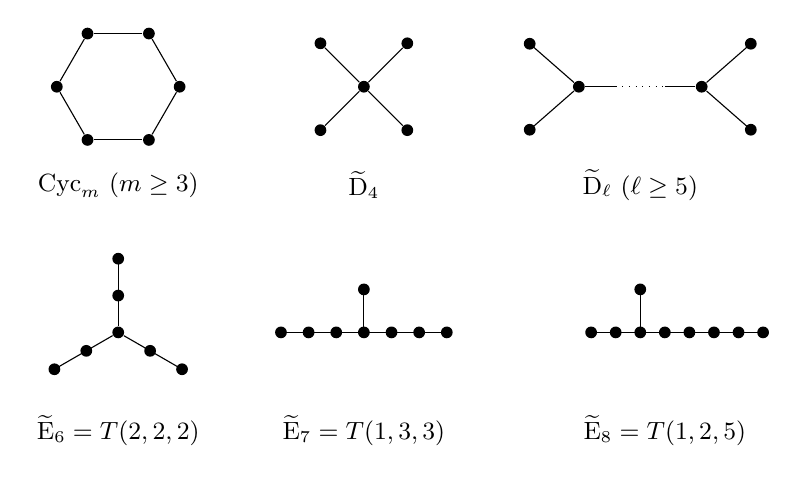
\begin{tikzpicture}[scale=.78, every node/.style={font=\small}, v/.style={circle,fill,inner sep=1.5pt}]
\foreach \i in {0,...,5} {\node[v] (c\i) at ({60*\i}:1) {};}
\foreach \i/\j in {0/1,1/2,2/3,3/4,4/5,5/0} {\draw (c\i)--(c\j);}
\node at (0,-1.6) {$\Cyc_m\ (m\geq3)$};
\begin{scope}[xshift=4cm]
\node[v] (d) at (0,0) {};
\foreach \i/\a in {1/45,2/135,3/225,4/315}{\node[v] (d\i) at (\a:1) {};\draw(d)--(d\i);}
\node at (0,-1.6) {$\widetilde{\typ D}_4$};
\end{scope}
\begin{scope}[xshift=8.5cm]
\node[v] (l) at (-1,0) {};\node[v] (r) at (1,0) {};
\draw (l)--(-.4,0);\draw[dotted](-.4,0)--(.4,0);\draw(.4,0)--(r);
\foreach \x/\name in {-1/l,1/r}{\foreach \y in {-1,1}{\node[v] at (\x*1.8,\y*.7) {};\draw (\name)--(\x*1.8,\y*.7);}}
\node at (0,-1.6) {$\widetilde{\typ D}_\ell\ (\ell\geq5)$};
\end{scope}
\begin{scope}[yshift=-4cm]
\node[v] (e) at (0,0) {};
\foreach \a in {90,210,330}{\foreach \t in {1,2}{\node[v] at (\a:{.6*\t}) {};}\draw(e)--(\a:1.2);}
\node at (0,-1.6) {$\widetilde{\typ E}_6=T(2,2,2)$};
\end{scope}
\begin{scope}[xshift=4cm,yshift=-4cm]
\foreach \i in {-3,...,3}{\node[v] at (.45*\i,0) {};}
\draw(-1.35,0)--(1.35,0);\draw(0,0)--(0,.7);\node[v] at (0,.7) {};
\node at (0,-1.6) {$\widetilde{\typ E}_7=T(1,3,3)$};
\end{scope}
\begin{scope}[xshift=8.5cm,yshift=-4cm]
\foreach \i in {-2,...,5}{\node[v] at (.4*\i,0) {};}
\draw(-.8,0)--(2,0);\draw(0,0)--(0,.7);\node[v] at (0,.7) {};
\node at (.4,-1.6) {$\widetilde{\typ E}_8=T(1,2,5)$};
\end{scope}
\end{tikzpicture}
\caption{The graphs in Corollary D. The first drawing represents any cycle;
the dotted segment in the $\widetilde{\typ D}$ drawing represents a path,
whose two endpoints are distinct. All edges have weight 1.}
\label{fig:smith}
\end{figure}

\section{Coordinate Root Systems and their bases}\label{sec:models}

We will give coordinates with the standard Euclidean inner product. In
each case the ambient space is the span specified below, rather than a
larger coordinate space. Root bases have indices starting at 0; coordinate
vectors $\Zu_i$ have indices starting at 1. Every sign in a set of the
form $\{\pm\Zu_i\pm\Zu_j\}$ is chosen independently.
Unqualified coordinate indices range over the coordinates of the stated
ambient space.

\subsection{The classical systems}

For the ranges in \eqref{eq:list}, define
\begin{align*}
 \Phi(\typ A_\ell)&=\{\Zu_i-\Zu_j:1\leq i\ne j\leq\ell+1\},
 &V(\typ A_\ell)&=\{\Zx:\textstyle\sum_i\Zx(i)=0\},\\
 \Phi(\typ B_\ell)&=\{\pm\Zu_i:1\leq i\leq\ell\}
             \cup\{\pm\Zu_i\pm\Zu_j:i<j\},
 &V(\typ B_\ell)&=\re^\ell,\\
 \Phi(\typ C_\ell)&=\{\pm2\Zu_i:1\leq i\leq\ell\}
             \cup\{\pm\Zu_i\pm\Zu_j:i<j\},
 &V(\typ C_\ell)&=\re^\ell,\\
 \Phi(\typ D_\ell)&=\{\pm\Zu_i\pm\Zu_j:1\leq i<j\leq\ell\},
 &V(\typ D_\ell)&=\re^\ell.
\end{align*}
We also use the displayed $\typ C$ model at rank 2 when discussing its
coincidence with $\typ B_2$. The proposed bases are
\begin{align}
 \typ A_\ell:\quad&\alpha_i=\Zu_{i+1}-\Zu_{i+2}
                    &&(0\leq i<\ell);\nonumber\\
 \typ B_\ell:\quad&\alpha_i=\Zu_{i+1}-\Zu_{i+2}
                    &&(0\leq i<\ell-1),&\alpha_{\ell-1}&=\Zu_\ell;\nonumber\\
 \typ C_\ell:\quad&\alpha_i=\Zu_{i+1}-\Zu_{i+2}
                    &&(0\leq i<\ell-1),&\alpha_{\ell-1}&=2\Zu_\ell;\nonumber\\
 \typ D_\ell:\quad&\alpha_i=\Zu_{i+1}-\Zu_{i+2}
                    &&(0\leq i<\ell-1),&\alpha_{\ell-1}&=\Zu_{\ell-1}+\Zu_\ell.
 \label{eq:classical-bases}
\end{align}

\begin{lemma}\label{lem:classical}
For $\ell\geq1$ in type $\typ A$, $\ell\geq2$ in types $\typ B,\typ C$,
and $\ell\geq4$ in type $\typ D$, the displayed sets are Root Systems in
the displayed spaces. The vectors in \eqref{eq:classical-bases} are bases,
and their Cartan matrices are exactly Mathlib's matrices of the same type.
\end{lemma}
\begin{proof}
All the sets are finite and have no zero. In each set, two vectors on one
line differ by sign: their supports and the equal absolute values on a
two-coordinate support determine this, while an axis has only its displayed
pair of roots. For a root $\Zu_i-\Zu_j$, reflection interchanges
coordinates $i,j$. For $\Zu_i+\Zu_j$, it interchanges those coordinates
and changes both signs. For an axis root, reflection changes the sign of
that coordinate, independent of whether the root is $\Zu_i$ or $2\Zu_i$.
Negating a root leaves its reflection unchanged. Coordinate permutations
preserve the $\typ A$ set and its zero-sum space. Signed coordinate
permutations preserve each of the $\typ B,\typ C,\typ D$ sets.
These descriptions verify closure under every root reflection.

The pairing coefficient with a root of squared length 2 is its inner
product with the other root, an integer. In type $\typ B$, a root of
squared length 1 gives twice an integer coordinate. In type $\typ C$,
pairing against $\pm2\Zu_i$, whose squared length is 4, gives
$\pm\Zx(i)$, also an integer. Thus the crystallographic condition holds.

We will verify the base property by displaying the positive roots. Every
root not on these lists is the negative of one on the lists. Empty sums
below have value zero. In all four types, for $i<j$,
\[
 \Zu_i-\Zu_j=\sum_{k=i-1}^{j-2}\alpha_k.
\]
In type $\typ A$ these exhaust one root from each pair of signs.
In type $\typ B$ the remaining choices are
\[
 \Zu_i=\sum_{k=i-1}^{\ell-1}\alpha_k,\qquad
 \Zu_i+\Zu_j=\sum_{k=i-1}^{j-2}\alpha_k+
                        2\sum_{k=j-1}^{\ell-1}\alpha_k.
\]
In type $\typ C$ they are
\[
 2\Zu_i=2\sum_{k=i-1}^{\ell-2}\alpha_k+\alpha_{\ell-1},\qquad
 \Zu_i+\Zu_j=\sum_{k=i-1}^{j-2}\alpha_k+
              2\sum_{k=j-1}^{\ell-2}\alpha_k+\alpha_{\ell-1}.
\]
In type $\typ D$, for $i<j\leq\ell-1$, they are
\[
 \Zu_i+\Zu_j=\sum_{k=i-1}^{j-2}\alpha_k+
  2\sum_{k=j-1}^{\ell-3}\alpha_k+\alpha_{\ell-2}+\alpha_{\ell-1},
\]
and for $i<\ell$ they are
\[
 \Zu_i+\Zu_\ell=\sum_{k=i-1}^{\ell-3}\alpha_k+\alpha_{\ell-1}.
\]
Each formula follows by telescoping the consecutive differences.
For $\Zu_i+\Zu_j$ with $j\leq\ell-1$, the identity
$\alpha_{\ell-2}+\alpha_{\ell-1}=2\Zu_{\ell-1}$ supplies the endpoint.
For $\Zu_i+\Zu_\ell$, we use only
$\alpha_{\ell-1}=\Zu_{\ell-1}+\Zu_\ell$.
These are nonnegative integer expansions of every indicated root.

The $\typ A$ roots span the zero-sum space: a vector in that space is
$\sum_{i=1}^{\ell}\Zx(i)(\Zu_i-\Zu_{\ell+1})$.
The axis roots span the $\typ B$ and $\typ C$ spaces. The $\typ D$ roots
span since, for $i\ne j$,
$2\Zu_i=(\Zu_i+\Zu_j)+(\Zu_i-\Zu_j)$.
The expansions prove that the $\ell$ displayed simple roots span these
$\ell$-dimensional spaces, so they are independent. Thus they are
bases in the root sense.

Finally, consecutive differences have squared norm 2 and inner product
$-1$; nonconsecutive differences have disjoint support. In type $\typ B$
the last squared norm is 1 and its inner product with its predecessor is
$-1$, giving entries $-2,-1$ in that order. In type $\typ C$ the last
squared norm is 4 and that inner product is $-2$, giving entries $-1,-2$.
In type $\typ D$ the final sum has squared norm 2, is orthogonal to
$\Zu_{\ell-1}-\Zu_\ell$, and has inner product $-1$ with
$\Zu_{\ell-2}-\Zu_{\ell-1}$; its other inner products are zero.
Substitution in \eqref{eq:pairing} gives every entry specified in
Section~\ref{sec:cartan}.
\end{proof}

\subsection{\texorpdfstring{The three $\typ E$ systems}{The three E systems}}

Define the lattice
\begin{equation}\label{eq:E-lattice}
 L=\{\Zx\in\ints^8:\textstyle\sum_i\Zx(i)\in2\ints\}
 \ \cup\
 \{\Zx\in(\ints+\tfrac12)^8:\textstyle\sum_i\Zx(i)\in2\ints\}.
\end{equation}
Here ``lattice'' will mean an additive subgroup generated by a real basis;
we will prove that assertion for $L$ below. Put
\begin{align*}
 \Phi(\typ E_8)&=\{\pm\Zu_i\pm\Zu_j:i<j\}\ \cup\
 \{\tfrac12\textstyle\sum_{i=1}^8\epsilon(i)\Zu_i:
       \epsilon(i)\in\{1,-1\},\ \prod_i\epsilon(i)=1\},\\
 V(\typ E_7)&=\{\Zx\in\re^8:\Zx(7)+\Zx(8)=0\},\\
 V(\typ E_6)&=\{\Zx\in\re^8:\Zx(6)=\Zx(7)=-\Zx(8)\},\\
 \Phi(\typ E_j)&=\Phi(\typ E_8)\cap V(\typ E_j)\qquad(j=6,7),
 \qquad V(\typ E_8)=\re^8.
\end{align*}
The eight simple roots, with Mathlib's zero-based ordering, are
\begin{equation}\label{eq:E-base}
 \begin{split}
 \alpha_0&=\tfrac12(\Zu_1+\Zu_8-\Zu_2-\Zu_3-\Zu_4-\Zu_5-\Zu_6-\Zu_7),\\
 \alpha_1&=\Zu_1+\Zu_2,\qquad
 \alpha_i=\Zu_i-\Zu_{i-1}\quad(2\leq i\leq7).
 \end{split}
\end{equation}
The notation in the last formula uses coordinate indices: it gives
$\alpha_2=\Zu_2-\Zu_1$, $\alpha_3=\Zu_3-\Zu_2$, up to
$\alpha_7=\Zu_7-\Zu_6$. We use the first $j$ vectors for type $\typ E_j$.

\begin{lemma}\label{lem:even-lattice}
The set $L$ in \eqref{eq:E-lattice} is an additive subgroup. Inner products
of its elements are integers, and squared norms are even integers. Its
vectors of squared norm 2 are exactly $\Phi(\typ E_8)$.
\end{lemma}
\begin{proof}
Write $L_0=\{\Zx\in\ints^8:\sum_i\Zx(i)\text{ is even}\}$ and
$\Zv=\tfrac12\sum_i\Zu_i$. Then $L=L_0\cup(L_0+\Zv)$
and $2\Zv\in L_0$. Thus addition and negation preserve $L$.
For $\Zx,\Zy\in L_0$, $\ip{\Zx}{\Zy}$ is an integer and
$\ip{\Zx}{\Zv}=\sum_i\Zx(i)/2$ is an integer; also $\lsq{\Zv}=2$.
Expanding inner products proves integrality on both cosets.
For $\Zx\in L_0$,
$\lsq{\Zx}\equiv\sum_i\Zx(i)\equiv0\pmod2$.
For $\Zx+\Zv\in L_0+\Zv$,
\[
 \lsq{\Zx+\Zv}=\sum_{i=1}^8\Zx(i)(\Zx(i)+1)+2\in2\ints.
\]
A nonzero lattice vector thus has squared norm at least 2. An integer
vector of norm squared 2 has exactly two nonzero coordinates, both $\pm1$.
A vector in the half-integer coset has all eight absolute coordinates at
least $1/2$. Equality at norm squared 2 forces all to be $1/2$.
Its coordinate sum is $4-t$, where $t$ is the number of negative signs;
the sum is even precisely when $t$ is even. This is exactly the displayed
list of roots.
\end{proof}

\begin{lemma}\label{lem:minimal-base}
Let $L$ be an additive subgroup of a Euclidean space, every nonzero element
of which has squared norm at least $b>0$. Let
$\alpha_0,\ldots,\alpha_{m-1}$ be a real basis generating $L$ over
$\ints$, with $\ip{\alpha_i}{\alpha_j}\leq0$ for $i\ne j$.
Every element of $L$ of squared norm $b$ has either all nonnegative or
all nonpositive integer coefficients in this basis.
\end{lemma}
\begin{proof}
Split its integer coefficient vector into its positive and negative parts,
writing the element as $\Zv-\Zw$, where both parts are nonnegative
combinations of disjoint subsets of the basis. Then
$\ip{\Zv}{\Zw}\leq0$. If both parts were nonzero, we would have
\[
 b=\lsq{\Zv-\Zw}=\lsq{\Zv}+\lsq{\Zw}-2\ip{\Zv}{\Zw}\geq2b,
\]
a contradiction. Thus one part is zero.
\end{proof}

\begin{lemma}\label{lem:E}
The sets $\Phi(\typ E_j)$, $j=6,7,8$, are Root Systems in their specified
spaces. Their bases are the first $j$ vectors in \eqref{eq:E-base}, and
their Cartan matrices are exactly \ml{CartanMatrix.E j}.
\end{lemma}
\begin{proof}
All the listed simple roots lie in $L$ and have squared norm 2. Given
$\Zx\in\re^8$, its coefficients in \eqref{eq:E-base} are
\begin{equation}\label{eq:E-coeff}
 \begin{split}
 c(0)&=2\Zx(8),\qquad
 c(1)=\tfrac12\sum_{i=1}^8\Zx(i)+2\Zx(8),\\
 c(2)&=c(1)+\Zx(8)-\Zx(1),\\
 c(k)&=\sum_{i=k}^7\Zx(i)+(8-k)\Zx(8)\quad(3\leq k\leq7).
 \end{split}
\end{equation}
Substitution gives coordinate 8 equal to $c(0)/2$, coordinate 1 equal
to $c(0)/2+c(1)-c(2)$, coordinate 2 equal to
$-c(0)/2+c(1)+c(2)-c(3)$, coordinates $3\leq i\leq6$ equal to
$-c(0)/2+c(i)-c(i+1)$, and coordinate 7 equal to $-c(0)/2+c(7)$.
These are exactly the coordinates of $\Zx$, proving the inversion formula
and linear independence. If $\Zx\in L$, then $c(0),c(1)$ are integers,
$\Zx(8)-\Zx(1)$ is an integer, and each summand
$\Zx(i)+\Zx(8)$ in $c(k)$ is an integer. Thus all coefficients are
integers, so these roots generate $L$.

The conditions for $V(\typ E_7)$ and $V(\typ E_6)$ are respectively
$c(7)=0$ and $c(7)=c(6)=0$. Thus their lattice intersections are
generated by the first seven and the first six simple roots. They also
span those subspaces, which have dimensions 7 and 6. Direct inner products
in \eqref{eq:E-base} give diagonal 2 and inner product $-1$ exactly on
$\{0,2\},\{1,3\},\{2,3\},\{3,4\},\ldots,\{6,7\}$.
To check the exceptional first vector, its coordinates at 1 and 8 are
$1/2$ and those at 2 through 7 are $-1/2$, so its inner product with
$\alpha_1$ is zero, with $\alpha_2$ is $-1$, and with
$\alpha_3,\ldots,\alpha_7$ is zero. The remaining products follow
from the two-coordinate supports of the displayed differences and sum.
Thus all off-diagonal inner products are nonpositive, and
Lemma~\ref{lem:minimal-base}, with $b=2$, proves the root base property
for $L$ and for each sublattice intersection.

For a root $\alpha$ of norm squared 2, reflection takes
$\Zx\in L$ to $\Zx-\ip{\Zx}{\alpha}\alpha\in L$, since the inner
product is an integer. Reflection preserves the norm, so it permutes the
norm-2 vectors. If both vectors lie in one of the specified subspaces,
their reflected vector remains there. Thus all three sets are closed under
reflections and are crystallographic. Equal nonzero lengths give
reducedness, and their simple roots prove spanning. Finally, denominator
2 in \eqref{eq:pairing} makes the Cartan entries exactly the inner products
just calculated, which are Mathlib's $\typ E_j$ entries.
\end{proof}

\subsection{\texorpdfstring{The $\typ F_4$ system}{The F4 system}}

In $\re^4$ put
\begin{equation}\label{eq:F-roots}
 \Phi(\typ F_4)=\{\pm\Zu_i\pm\Zu_j:i<j\}
 \cup\{\pm\Zu_i:1\leq i\leq4\}
 \cup\{\tfrac12(\epsilon(1)\Zu_1+\epsilon(2)\Zu_2+
                    \epsilon(3)\Zu_3+\epsilon(4)\Zu_4):\epsilon(i)=\pm1\}.
\end{equation}
Its proposed ordered base is
\begin{equation}\label{eq:F-base}
 \alpha_0=\Zu_2-\Zu_3,\quad
 \alpha_1=\Zu_3-\Zu_4,\quad
 \alpha_2=\Zu_4,\quad
 \alpha_3=\tfrac12(\Zu_1-\Zu_2-\Zu_3-\Zu_4).
\end{equation}

\begin{lemma}\label{lem:F}
The set \eqref{eq:F-roots} is a Root System with base \eqref{eq:F-base}
and Cartan matrix \texttt{CartanMatrix.F}\textsubscript{4}.
Its first two simple roots are long and its last two are short.
\end{lemma}
\begin{proof}
The squared lengths are 2 on the two-coordinate roots and 1 on the other
roots. Supports show there are no proportional roots except sign pairs;
the axes show spanning. Signed coordinate permutations preserve the set.
Reflections in the two-coordinate and axis roots are signed coordinate
permutations as in Lemma~\ref{lem:classical}.

It remains to check a half-coordinate root. Every such root is carried
to $\Zv=(\Zu_1+\Zu_2+\Zu_3+\Zu_4)/2$ by a diagonal sign change
preserving the set. An orthogonal transformation $\phi$ satisfies
$s_{\phi\alpha}=\phi s_\alpha\phi\inv$, by substitution in the reflection
formula. Thus it suffices to check $s_\Zv$ on all three kinds of
roots. Its formula is
\[
 s_\Zv\Zx=\Zx-\left(\sum_i\Zx(i)\right)\Zv.
\]
An axis vector $\Zu_i$ goes to $\Zu_i-\Zv$, a half-coordinate root;
its negative goes to the negative of that image. A two-coordinate root
with opposite signs is fixed. One with equal sign $\epsilon$ on
coordinates $i,j$ goes to $-\epsilon(\Zu_k+\Zu_l)$ on the other two
coordinates. For a half-coordinate root with $t$ plus signs, the
coordinate sum is $t-2$. For $t=0$ or 4 its image is its negative;
for $t=2$ it is fixed; for $t=1$ its image is the positive axis at its
unique plus sign; for $t=3$ its image is the negative axis at its unique
minus sign. This proves closure under every reflection.

Pairing against a long root is an inner product. With a half-coordinate
root this is a sum of two numbers $\pm1/2$, and with an integer root it
is an integer. Pairing against an axis root is twice a coordinate and
is an integer. Pairing against a half-coordinate root, of squared length
1, is twice the inner product. For an integer root that is a signed sum
of integer coordinates. For another half-coordinate root it is
$(4-2t)/2=2-t$, where $t$ counts differing signs. Thus all pairings
are integers.

The coefficients of a vector $\Zx$ in the ordered base are
\begin{equation}\label{eq:F-coeff}
 \bigl(\Zx(1)+\Zx(2),\quad 2\Zx(1)+\Zx(2)+\Zx(3),\quad
 3\Zx(1)+\Zx(2)+\Zx(3)+\Zx(4),\quad 2\Zx(1)\bigr).
\end{equation}
Substitution in \eqref{eq:F-base} proves this inversion formula and
independence. Orient a root with $\Zx(1)\ne0$ so that
$\Zx(1)>0$. If it is a half-coordinate root, these four coefficients
are integers in $[0,1],[0,2],[0,3],\{1\}$, respectively.
If $\Zx(1)=1$, the other coordinates have at most one nonzero entry,
equal to $1$ or $-1$. The coefficients are again nonnegative integers.
If $\Zx(1)=0$, orient the first nonzero coordinate among 2, 3, 4 to be
positive. There are at most two nonzero coordinates, each of absolute
value 1. Every prefix sum of these three coordinates is nonnegative:
after any initial zeros it starts with 1 and can subsequently decrease
by at most 1.
The coefficients in \eqref{eq:F-coeff} are those prefix sums and zero.
This proves the base property for every root.

The simple squared lengths are $(2,2,1,1)$ and the only nonzero
off-diagonal inner products are
$\ip{\alpha_0}{\alpha_1}=-1$,
$\ip{\alpha_1}{\alpha_2}=-1$ and
$\ip{\alpha_2}{\alpha_3}=-1/2$.
Equation~\eqref{eq:pairing} gives exactly the displayed $\typ F_4$ matrix.
\end{proof}

\subsection{\texorpdfstring{The $\typ G_2$ system}{The G2 system}}

In the plane $V=\{\Zx\in\re^3:\Zx(1)+\Zx(2)+\Zx(3)=0\}$ put
\begin{align}
 \Phi(\typ G_2)&=\{\Zu_i-\Zu_j:i\ne j\}\cup
      \{\pm(2\Zu_i-\Zu_j-\Zu_k):\{i,j,k\}=\{1,2,3\}\},
       \label{eq:G-roots}\\
 \alpha_0&=\Zu_1-2\Zu_2+\Zu_3,\qquad
 \alpha_1=\Zu_2-\Zu_3.                                      \label{eq:G-base}
\end{align}

\begin{lemma}\label{lem:G}
The set \eqref{eq:G-roots} is a Root System in $V$, with ordered base
\eqref{eq:G-base} and Cartan matrix
\texttt{CartanMatrix.G}\textsubscript{2}. Simple root 0 is long and
simple root 1 is short.
\end{lemma}
\begin{proof}
The six difference roots have squared length 2 and the six other roots
have squared length 6. Their coordinate patterns give six distinct sign
pairs, so they are reduced. Difference roots span $V$. Permuting
coordinates and negating all coordinates preserve the set.
A short-root reflection interchanges two coordinates. For the long root
$\beta=2\Zu_1-\Zu_2-\Zu_3$, a vector $\Zx\in V$ has
$\ip{\Zx}{\beta}=3\Zx(1)$, so
\[
 s_\beta\Zx=(-\Zx(1),\Zx(2)+\Zx(1),\Zx(3)+\Zx(1))
            =(-\Zx(1),-\Zx(3),-\Zx(2)).
\]
This preserves the set. Each other long root is a coordinate permutation
of $\beta$ or its negative; conjugating by that permutation proves closure
for each of them. A pairing against a short root is an integer inner
product, and a pairing against $\beta$ is $\Zx(1)$, an integer on the
root set. Permutation and sign give integrality against every long root.

In the order $(\alpha_0,\alpha_1)$, the positive coefficient pairs are
\begin{equation}\label{eq:G-coeff}
 (0,1),\ (1,1),\ (1,2),\ (1,0),\ (1,3),\ (2,3).
\end{equation}
The first three vectors are, in order,
$\Zu_2-\Zu_3,\Zu_1-\Zu_2,\Zu_1-\Zu_3$.
The last three are
$\Zu_1-2\Zu_2+\Zu_3,\Zu_1+\Zu_2-2\Zu_3,2\Zu_1-\Zu_2-\Zu_3$.
Together with their negatives these are all twelve roots.
The simple Gram matrix is $\pmat{6&-3\\-3&2}$, whose determinant is 3,
so the two roots are independent. Formula~\eqref{eq:G-coeff} proves the
base property, and dividing its columns by the respective half squared
lengths gives $\pmat{2&-3\\-1&2}$, as required.
\end{proof}

\begin{lemma}\label{lem:models-irreducible}
Every coordinate Root System constructed in this section, in the parameter
ranges stated for its construction, is indecomposable.
\end{lemma}
\begin{proof}
The calculated simple-root nonorthogonality graph is connected in every
case. If all roots were partitioned into two orthogonal nonempty subsets,
each pair of nonorthogonal simple roots would lie in the same part.
Following paths puts all simple roots in one part. Every root in the other
part would be perpendicular to their spanning set, and would be zero,
a contradiction. This includes a one-element base, since it already spans.
\end{proof}

\section{From Root Systems to Mathlib and back}\label{sec:bridge}

\begin{lemma}\label{lem:pairing-construction}
Let $\Phi$ be a Root System in a Euclidean space $V$.
It defines a finite, crystallographic, reduced root pairing over $\re$
which is a root system in Mathlib's sense. If $\Phi$ is nonempty, its
indecomposability is equivalent to Mathlib's irreducibility.
\end{lemma}
\begin{proof}
Use the finite index set $\iota=\Phi$, the two spaces $V,V$, and the
bilinear form \texttt{inner}\textsubscript{l}\,$V$ for their inner
product (the identifier is \texttt{inner} followed by Unicode subscript l).
It is injective in each argument: if a difference $\Zz$ pairs to zero
with every vector, pair it with $\Zz$ to obtain $\lsq{\Zz}=0$,
so $\Zz=0$. Finite dimensionality and
\ml{LinearMap.IsPerfPair.of_injective} make it a perfect pairing.
The root embedding is inclusion and the coroot
embedding sends $\alpha$ to
\[
 \alpha^\vee=\frac{2\alpha}{\lsq{\alpha}}.
\]
This map is injective: applying the same operation twice returns the
original nonzero vector. Its pairing with its root is 2.
Let the reflection permutation on $\iota$ be $s_\alpha$ restricted to
$\Phi$; it is a permutation since it is an involution.
The root reflection identity is the defining formula. For the coroot
identity, orthogonality of $s_\alpha$ gives
\[
 (s_\alpha\beta)^\vee=s_\alpha(\beta^\vee)
    =\beta^\vee-\ip{\alpha}{\beta^\vee}\alpha^\vee.
\]
These are exactly the two identities in the structure constructor
\ml{RootPairing}. Its pairing is \eqref{eq:pairing}; condition (a) of
Definition~\ref{def:roots}, with the two roots interchanged, supplies
\ml{IsCrystallographic}. A dependent pair of nonzero vectors over $\re$
is proportional; condition (b) supplies \ml{IsReduced}.
Roots span by assumption and their nonzero scalar multiples, the coroots,
have the same span. Thus \ml{IsRootSystem} holds.

We will check irreducibility explicitly. Suppose $W$ is a subspace
invariant under every $s_\alpha$. If some $\Zw\in W$ has
$\ip{\Zw}{\alpha}\ne0$, then $\Zw-s_\alpha\Zw$ is a nonzero multiple
of $\alpha$, so $\alpha\in W$. Otherwise $\alpha\in W^\perp$.
Thus every root lies in $W$ or $W^\perp$. If $W\ne0$ and $W\ne V$,
both sets of roots are nonempty: if all roots lay in one, their span would
force the other subspace to be zero. They are disjoint since a nonzero
vector cannot belong to $W\cap W^\perp$, and they are mutually orthogonal.
This contradicts indecomposability. The root and coroot reflections on
our two copies of $V$ are the same orthogonal maps, so both irreducibility
conditions hold. Nonemptiness of $\Phi$ gives $V\ne0$, as required by
Mathlib's definition. Alternatively, \ml{RootPairing.IsIrreducible.mk'}
supplies the coroot half of this argument.

Conversely, if roots partition into two nonempty orthogonal sets, the
span of either is a nonzero proper subspace. Reflections belonging to
that set preserve its span; reflections belonging to the other set fix
it pointwise. This is a proper invariant subspace, contradicting
\ml{IsIrreducible}.
\end{proof}

The constructor \ml{RootPairing.ofBilinear} is not a constructor for an
arbitrary prescribed finite subset. It takes \emph{all} reflective vectors
of its form. For a positive definite real form, every nonzero vector is
reflective, because its squared norm is nonzero and divides every real
number. In particular, using it directly over $\re$ in positive dimension
would give an infinite index set. The direct structure construction in
Lemma~\ref{lem:pairing-construction} is the interface we actually use.

\begin{lemma}\label{lem:similarity}
Let $\Phi,\Psi$ be nonempty Root Systems with bases
$(\alpha_i)_{i\in I}$ and $(\beta_i)_{i\in I}$ indexed by the same finite
set. Suppose their Cartan matrices coincide and their common nonzero
off-diagonal support is connected. The linear map taking each $\alpha_i$
to $\beta_i$ is a similarity of the ambient Euclidean spaces.
If that linear map sends $\Phi$ onto $\Psi$, it is a similarity of
the Root Systems themselves.
\end{lemma}
\begin{proof}
Write $q(i)=\lsq{\alpha_i}$ and $r(i)=\lsq{\beta_i}$.
Symmetry of the two inner products gives
\[
 M(i,j)q(j)=M(j,i)q(i),\qquad
 M(i,j)r(j)=M(j,i)r(i).
\]
On an edge, both matrix entries are nonzero. Dividing shows
$r(i)/q(i)=r(j)/q(j)$. Connectedness makes this ratio a single positive
constant $a$. For every pair, including nonedges and equal indices,
\[
 \ip{\beta_i}{\beta_j}=\tfrac12 M(i,j)r(j)
                     =a\ip{\alpha_i}{\alpha_j}.
\]
Expanding arbitrary vectors in the two bases proves the similarity
identity. The last assertion follows from the given equality of root
sets under the map. Only one common scaling factor
is used; short and long roots cannot be rescaled independently.
\end{proof}

\begin{theoremB}
\textup{\cite[Remark 3.11]{CGSS}}
Every nonempty indecomposable Root System of Definition~\ref{def:roots}
is, after one common positive rescaling, isometric to exactly one of the
coordinate Root Systems
\[
 \typ A_\ell\ (\ell\geq1),\quad
 \typ B_\ell\ (\ell\geq2),\quad
 \typ C_\ell\ (\ell\geq3),\quad
 \typ D_\ell\ (\ell\geq4),\quad
 \typ E_6,\typ E_7,\typ E_8,\typ F_4,\typ G_2.
\]
Exactly the $\typ B,\typ C,\typ F,\typ G$ systems have two root lengths.
The rank-2 model $\typ C_2$ is similar to $\typ B_2$; we omit it
from the uniqueness list. Every Root System is an orthogonal sum
of these indecomposable systems, with an independent scale for each
nonzero orthogonal component.
\end{theoremB}
\begin{proof}
Apply Lemma~\ref{lem:pairing-construction}. The theorem
\ml{RootPairing.nonempty_base} supplies a base $b$ for this finite,
reduced, crystallographic root system over $\re$.
Its support is nonempty by \ml{RootPairing.Base.support_nonempty},
since the root index set is nonempty and $2\ne0$ in $\re$.
The declarations
\ml{RootPairing.Base.cartanMatrix_isFiniteCartan} and
\ml{RootPairing.Base.cartanMatrix_isIndecomposable} give exactly the
hypotheses of Theorem A. Apply it and reindex the base by its resulting
bijection.

Section~\ref{sec:models} supplies a coordinate Root System with a root
base having the resulting matrix. Apply Lemma~\ref{lem:pairing-construction}
to that model. Use \ml{RootPairing.Base.mk'} with the verified
independence and signed expansions to obtain a Mathlib base $b_2$.
Let $e$ be the resulting equivalence between
the two base supports and take
$f=b.\ml{toWeightBasis.equiv}\ b_2.\ml{toWeightBasis}\ e$.
This linear equivalence takes each selected simple root to its model
simple root, by \ml{Module.Basis.equiv_apply} and
\ml{RootPairing.Base.toWeightBasis_apply}.
Apply \ml{RootPairing.Base.apply_mem_range_root_of_cartanMatrixEq}
to $f$, and then to $f\inv$ with $e\inv$ and the Cartan equality
reversed. The first application gives $f(\Phi)\sbs\Psi$ and the second
gives $f\inv(\Psi)\sbs\Phi$. Thus $f(\Phi)=\Psi$.
Lemma~\ref{lem:similarity} makes $f$ an isometry after one common
rescaling. Section~\ref{sec:interface} states all the hypotheses
of these declarations; the field, finiteness, spanning, reducedness and
crystallographic hypotheses have all been checked above.

For uniqueness we will use invariants of the Root System itself, so no
conjugacy theorem for bases is needed. Rank, number of roots, the number
of distinct lengths, and the numbers of short and long roots are invariant
under similarity. We will prove their values in
Lemma~\ref{lem:counts} and record them in Table~\ref{tab:roots}.
Among one-length systems, at rank $\ell$ the classical root counts are
$\ell(\ell+1)$ and $2\ell(\ell-1)$; these are equal only at $\ell=3$,
outside our $\typ D$ range. At ranks 6, 7 and 8, the exceptional counts
72, 126 and 240 differ from both classical counts, which are respectively
$(42,60)$, $(56,84)$ and $(72,112)$.
Among two-length systems, $\typ G_2$ has squared-length ratio 3;
all the others have ratio 2. Type $\typ F_4$ has 48 roots in rank 4,
where $\typ B_4,\typ C_4$ have 32. For $\ell\geq3$, the numbers of
short roots in $\typ B_\ell,\typ C_\ell$ are $2\ell$ and
$2\ell(\ell-1)$ and are unequal. Rank separates parameters.
These invariants distinguish every entry of the list.

In rank 2 the linear map with matrix
$\pmat{1&1\\-1&1}$ takes the four axis roots of $\typ B_2$ to
the four two-coordinate roots of $\typ C_2$ and the other four roots
to its axis roots. Its transpose times itself is $2I$, so it is the
required similarity. The displayed coordinate lengths establish the
assertion about which systems have two lengths.

Finally, join two roots whenever they have nonzero inner product.
Connected components of this finite graph are mutually orthogonal.
Each is closed under reflection in one of its own roots. Indeed, if
$\ip{\alpha}{\beta}\ne0$, then
$\ip{\alpha}{s_\alpha\beta}=-\ip{\alpha}{\beta}\ne0$;
so the reflected root is in the same component as $\alpha$;
if that inner product is zero, $s_\alpha\beta=\beta$.
Thus each component is a Root System in its span. These spans give an
orthogonal direct sum since the roots span the ambient space. The
classification applies separately to each component, with a separate
positive scale. The zero space contributes no component.
\end{proof}

\section{Lengths, lines, and the matrix equations}\label{sec:lines}

\begin{lemma}\label{lem:angles}
Let $\Phi$ be a Root System. For every pair $\alpha,\beta\in\Phi$
which is neither perpendicular nor proportional, we have
\[
 \frac{4\ip{\alpha}{\beta}^2}{\lsq{\alpha}\lsq{\beta}}\in\{1,2,3\}.
\]
The ratio of the longer length to the shorter length and the acute angle
between their lines are respectively
$(1,60^\circ)$, $(\sqrt2,45^\circ)$ or $(\sqrt3,30^\circ)$.
For any length $a>0$ which occurs in $\Phi$, the roots of length $a$
are a Root System in their span, and this subsystem is an orthogonal sum
of systems similar to $\typ A_\ell$ ($\ell\geq1$), $\typ D_\ell$
($\ell\geq4$), or $\typ E_6,\typ E_7,\typ E_8$.
\end{lemma}
\begin{proof}
For such a pair, the two numbers $2\ip{\alpha}{\beta}/\lsq{\alpha}$ and
$2\ip{\alpha}{\beta}/\lsq{\beta}$ are nonzero integers of the same
sign. Their product is positive and, by strict Cauchy-Schwarz for a
nonproportional pair, is less than 4. The unordered pair of their absolute
values is thus $(1,1)$, $(1,2)$ or $(1,3)$. Dividing the two
pairings gives the ratio of squared lengths or its reciprocal. Their
product is four times the squared cosine of the acute line angle, giving
the stated pairs.

The roots of fixed length are finite, nonzero and span their own span;
integrality and reducedness are inherited. A reflection in one of those
roots maps each of them to a root of the original system and preserves
length. Its formula also keeps the vector in their span. This verifies
all Root System conditions. Such a subsystem can be decomposable. The
classification in Theorem B makes it an orthogonal sum of one-length
systems of types $\typ A,\typ D,\typ E$, because every unequal-length
type in that theorem actually has two lengths.
\end{proof}

\begin{lemma}\label{lem:counts}
The coordinate Root Systems in Section~\ref{sec:models} have the root
counts, length counts and line counts in Table~\ref{tab:roots}.
\end{lemma}
\begin{proof}
There are $\ell(\ell+1)$ ordered distinct-coordinate differences in
$\typ A_\ell$. There are $4\binom\ell2=2\ell(\ell-1)$ signed
two-coordinate roots in each of $\typ B_\ell,\typ C_\ell,\typ D_\ell$.
The first two types have an additional $2\ell$ axis roots; these are
short in $\typ B$ and long in $\typ C$.

For $\typ E_8$ there are $4\binom82=112$ integer roots.
Seven half-coordinate signs can be chosen arbitrarily and the eighth is
then determined by the product condition, giving $2^7=128$ more roots.
In $\typ E_7$, integer roots either use two coordinates among the first
six, giving 60, or are $\pm(\Zu_7-\Zu_8)$, giving 2. In a half-coordinate
root the last two signs are opposite, and the product of the first six
is $-1$. Choose five of those signs and the last sign freely, giving
$2^5\cdot2=64$. Thus the total is 126.
In $\typ E_6$, an integer root cannot have any nonzero coordinate among
6, 7, 8: the subspace conditions would make all three nonzero, although
an integer root has only two nonzero coordinates. Thus there are
$4\binom52=40$. For half-coordinate roots, the first five signs
determine sign 8 by their product; signs 6 and 7 are both its negative.
This gives $2^5=32$ and a total of 72.

In $\typ F_4$ there are 24 two-coordinate long roots, 8 short axis roots
and 16 short half-coordinate roots. In $\typ G_2$ there are 6 short
differences and 6 long roots. All these enumerations use disjoint
coordinate patterns, so nothing is counted twice. Reducedness and
closure under negation give exactly two roots on every root line.
Dividing each root count by 2 gives the line count.
\end{proof}

\begin{lemma}\label{lem:tight-frame}
Let $\Phi$ be a nonempty indecomposable Root System in an
$n$-dimensional Euclidean space, and let $\cL$ be its $N$ lines.
Choose any unit vector $\Zv_L$ on each line $L$. Then
\begin{equation}\label{eq:frame}
 \cF:=\sum_{L\in\cL}\Zv_L\Zv_L^T=\frac{N}{n}I.
\end{equation}
Here $\Zv_L\Zv_L^T$ means the operator
$\Zx\mapsto\ip{\Zv_L}{\Zx}\Zv_L$, which is independent of the sign choice.
Unit vectors satisfying \eqref{eq:frame} form a \emph{tight frame}.
\end{lemma}
\begin{proof}
Every root reflection permutes the lines and is orthogonal, so conjugating
the sum by $s_\alpha$ leaves it unchanged. Thus $\cF$ commutes with every
$s_\alpha$. The $-1$-eigenspace of $s_\alpha$ is precisely $\re\alpha$,
so $\cF\alpha=t_\alpha\alpha$ for some real scalar $t_\alpha$.
Since $\cF$ is symmetric,
\[
 t_\alpha\ip{\alpha}{\beta}
   =\ip{\cF\alpha}{\beta}=\ip{\alpha}{\cF\beta}
   =t_\beta\ip{\alpha}{\beta}.
\]
Thus these scalars agree for nonorthogonal roots. Their nonorthogonality
graph is connected, since two unions of components would be an orthogonal
decomposition. All scalars have one value $t$. Roots span, so $\cF=tI$.
The trace of a unit rank-one operator is 1, as follows by summing its
diagonal entries in an orthonormal basis. Taking traces gives $nt=N$,
proving \eqref{eq:frame}.
\end{proof}

\begin{lemma}\label{lem:C-convention}
Let $N$ lines span an $n$-dimensional Euclidean space, with $n>0$.
Choose unit vectors on them, let $U$ have these vectors as columns, and
write $G=U^TU$. Define
\begin{equation}\label{eq:C-convention}
 C=2G-2I_N.
\end{equation}
For a real number $\theta$,
\[
 (C+2I_N)(C-\theta I_N)=0
 \quad\Longleftrightarrow\quad
 UU^T=\frac{N}{n}I_n\ \hbox{ and }\ \theta=\frac{2N}{n}-2.
\]
Both conditions are independent of the choices of signs.
\end{lemma}
\begin{proof}
Put $t=(\theta+2)/2$. Expanding the matrix product gives
$4(G^2-tG)$. If $UU^T=tI$, then $G^2=tG$. Conversely,
\[
 G^2-tG=U^T(UU^T-tI)U.
\]
The columns of $U$ span, so for any $\Zx,\Zy$ in the ambient space there
are coefficient vectors $\Zv,\Zw$ with $U\Zv=\Zx$ and $U\Zw=\Zy$.
If the displayed matrix vanishes then
$\Zx^T(UU^T-tI)\Zy=0$ for all $\Zx,\Zy$, so $UU^T=tI$.
Its trace is $N$, so $t=N/n$. Changing column signs replaces $U$ by
$UD_\epsilon$ for the diagonal sign matrix $D_\epsilon=\opk{diag}(\epsilon)$, with $D_\epsilon^2=I$.
It leaves $UU^T$ unchanged and conjugates $G$ and $C$ by $D_\epsilon$.
\end{proof}

Equation~\eqref{eq:C-convention} is our explicit convention for the
undefined matrix in Remark 3.11. It is the direct extension of the
convention preceding Theorem 3.7: vectors of squared norm 2 on the lines
have Gram matrix $2G=2I+C$. The source introduces this normalization
for any Root System. For two lengths we normalize representatives
\emph{line by line} to squared norm 2 to define this matrix; these
normalized representatives are not asserted to be a Root System.
The entries of $C$ need not be integers: at $45^\circ$ or $30^\circ$
they are $\pm\sqrt2$ or $\pm\sqrt3$. The identities below verify that
this convention gives every printed constant of Remark 3.11.
Choosing actual roots of unequal lengths instead would give a Gram
matrix with nonconstant diagonal, which cannot be $2I+C$ for a
zero-diagonal $C$.

\begin{theoremC}
\textup{\cite[Remark 3.11]{CGSS}}
With $C$ defined by \eqref{eq:C-convention}, all the following statements
hold. Nonperpendicular, nonproportional roots have the three length-ratio
and angle possibilities of Lemma~\ref{lem:angles}, and roots of any
occurring fixed length form a Root System in their span, which is an
orthogonal sum of systems similar to the one-length models
$\typ A_\ell$ ($\ell\geq1$), $\typ D_\ell$ ($\ell\geq4$),
$\typ E_6,\typ E_7,\typ E_8$.
For $n\geq2$, the $\typ B_n$ and $\typ C_n$ models give the same
$n^2$ lines in dimension $n$, with possible distinct-line angles
$90^\circ,60^\circ,45^\circ$, and
\[
 (C+2I)(C-2(n-1)I)=0.
\]
Type $\typ F_4$ gives 24 lines in dimension 4 with distinct-line angles
$90^\circ,60^\circ,45^\circ$, and
\[
 (C+2I)(C-10I)=0.
\]
Type $\typ G_2$ gives 6 lines in dimension 2 with distinct-line angles
$90^\circ,60^\circ,30^\circ$, and
\[
 (C+2I)(C-4I)=0.
\]
For $\typ B_2=\typ C_2$ as line systems, the angle $60^\circ$ does
not occur; for $n\geq3$ all three listed $\typ B_n$ angles occur.
A set of three lines pairwise at $45^\circ$ exists in $\re^3$ and is
not contained in the lines of any Root System.
\end{theoremC}
\begin{proof}
The first assertions are Lemma~\ref{lem:angles}.
The $\typ B_n$ and $\typ C_n$ axis roots lie on the same axes, and
their two-coordinate roots are identical. Thus their lines coincide.
Lemma~\ref{lem:counts} gives $n^2,24,6$ lines for the three cases.
The squared lengths in $\typ B,\typ C,\typ F$ have ratio 2, and those
in $\typ G$ have ratio 3. Lemma~\ref{lem:angles}, with the perpendicular
case included, proves the asserted allowed angle sets.
For $\typ B_n$ with $n\geq3$, the axes 1 and 2 give $90^\circ$,
axis 1 and $\Zu_1+\Zu_2$ give $45^\circ$, and
$\Zu_1+\Zu_2,\Zu_1+\Zu_3$ give $60^\circ$.
The same pairs are present in the $\typ C_n$ line set and in $\typ F_4$.
For $n=2$ there are only the two axes and the two diagonal lines; their
angles are $45^\circ$ or $90^\circ$.
In $\typ G_2$, the two short lines
$\Zu_1-\Zu_2,\Zu_1-\Zu_3$ give $60^\circ$;
the long root $2\Zu_1-\Zu_2-\Zu_3$ is perpendicular to
$\Zu_2-\Zu_3$ and makes a $30^\circ$ line angle with
$\Zu_1-\Zu_2$, since its inner product with that root is 3 and
the product of their lengths is $\sqrt{12}$.

The systems are indecomposable by Lemma~\ref{lem:models-irreducible}.
Apply Lemmas~\ref{lem:tight-frame} and~\ref{lem:C-convention}.
The values of $N/n$ are $n,6,3$; thus $\theta=2n-2,10,4$.
We will also give explicit coordinate sums verifying the frame identities
in Appendix~\ref{sec:data}.

For the final example put $c=1/\sqrt2$ and use the three unit vectors
\[
 \Zu_1,\qquad c\Zu_1+c\Zu_2,\qquad
 c\Zu_1+(1-c)\Zu_2+\sqrt{2c-1}\Zu_3.
\]
The radicand is positive. The squared norm of the third vector is
$c^2+(1-c)^2+2c-1=2c^2=1$.
Their pairwise inner products are $c,c,c^2+c(1-c)=c$, so the line angles
are all $45^\circ$. If roots on these lines belonged to a Root System,
every pair of their squared lengths would have ratio 2 in one order.
Choose one with minimal squared length $b$. Each of the other two must
then have squared length $2b$, but their equal lengths contradict their
$45^\circ$ angle by Lemma~\ref{lem:angles}. This proves noncontainment,
in any ambient dimension and without an irreducibility assumption.
\end{proof}

The same reasoning proves the equations of Theorem 3.7, independently of
its trace calculation. The values of $N/n$ for
$\typ A_n,\typ D_n,\typ E_6,\typ E_7,\typ E_8$ are
$(n+1)/2,n-1,6,9,15$, respectively. Thus their second constants are
$n-1,2(n-2),10,16,28$. In particular the printed $18$ for $\typ E_8$
is false; $28$ is required. In fact the squared-norm-2 Gram matrix
$2I+C$ has nonzero eigenvalue 30 under the frame identity, making the
corresponding $C$ eigenvalue 28.

\section{Interpretations and corrections of the sources}\label{sec:corrections}

We read \cite{CGSS} in its published form, in particular
pages 312--315. The following points are part of our statements.
\begin{enumerate}
\item The finite-type matrix assertion requires a nonempty index set.
 The empty matrix satisfies both Mathlib predicates and is a separate
 rank-zero case. For Root Systems we include nonemptiness in
 ``indecomposable'', matching the nontriviality in
 \ml{RootPairing.IsIrreducible}.
\item We use nonzero roots in Definition 3.9 and read the $S$ in its
 condition (b) as $\Sigma$. Zero is excluded by the definition's own
 proportionality condition, as explained in Section~\ref{sec:prelim}.
\item The opening of Remark 3.11 needs ``not proportional'' as well as
 ``not perpendicular''. Taking $\beta=\alpha$ gives product 4 and
 line angle $0^\circ$. Also, a length ratio is understood as longer
 divided by shorter; an ordered ratio can instead be a reciprocal.
\item A fixed-length subset is a Root System in \emph{its own span}.
 It need not span the original ambient space, and it can be decomposable.
 For example the long roots of $\typ B_2$ are two perpendicular sign
 pairs, so their subsystem is $\typ A_1\oplus\typ A_1$.
 For a failure of spanning, $\{\pm\Zu_1,\pm2\Zu_2\}$ is a Root
 System in $\re^2$, but its roots of length 1 span only one axis.
 Lemma~\ref{lem:angles} and Theorem C also state that these subsystems
 are orthogonal sums of the $\typ A,\typ D,\typ E$ models.
 We prove this part of Remark 3.11 from Theorem B, without using
 \cite[Theorem 3.10]{CGSS}; Theorem B does not depend on the assertion.
\item We define the matrix in Remark 3.11 by $C=2G-2I$ for unit
 representatives, extending the equal-length convention before
 Theorem 3.7. The source supplies no separate definition there.
 The resulting three equations agree with the printed ones. This is
 an explicit convention, not a claim that the unnormalized Gram matrix
 of unequal-length roots is $2I+C$.
\item The angle lists mean allowed angles. At rank 2, the
 $\typ B_n,\typ C_n$ list has no $60^\circ$ pair. At rank 1 there is
 one line, no pair of distinct lines and only one root length; its
 matrix is $C=[0]$. The unequal-length statement starts at rank 2.
\item The constant $18$ for $\typ E_8$ in Theorem 3.7 (p.~312) is an error
 of the paper. We correct it to $28$.
\item Theorem 3.8 is for finite connected simple graphs. We draw the
 graphs of its Figure 1 in our Figure~\ref{fig:smith}.
 The printed labels $A_n,D_n,E_6,E_7,E_8$ correspond respectively to
 our $\Cyc_{n+1},\widetilde{\typ D}_n,\widetilde{\typ E}_6,
 \widetilde{\typ E}_7,\widetilde{\typ E}_8$.
 Corollary D strengthens the source's one-way classification to an
 equivalence. The asterisk in each source drawing marks a vertex whose
 deletion leaves the finite diagram with the same type label; we omit
 the asterisks because we prove the basis assertion for every deletion,
 so also for those marked vertices. The deletion assertion
 holds for \emph{any} one vector, in the span of dimension $m-1$.
 Its notation $\re^n$ must refer to that span (or to a spanning
 realization), rather than an arbitrarily larger ambient space.
\end{enumerate}
Theorem 3.12 is outside the scope of this document; we prove it in
\ml{cgss/proofs/thm312/thm312.tex}. The three-line example immediately before it is
proved here. No classification theorem from \cite{CGSS} or \cite{BCN}
is used as a premise. In the Mathlib interface we additionally distinguish
the actual rank of \ml{CartanMatrix.A} from its docstring, and the
all-reflective-vectors constructor from a constructor for a prescribed
finite root set.

\section{Interface with Mathlib}\label{sec:interface}
\begingroup
\raggedright

We will distinguish library premises, available results that we do not use
as premises, and the missing statements proved here. All paths below are
relative to Mathlib at the commit stated in the introduction, the version
pinned in \ml{lake-manifest.json}, and we read the declarations there. We construct the coordinate
models here; we do not cite them as existing Mathlib declarations.

\subsection{Matrices and Rayleigh quotients}

The file \ml{Mathlib/LinearAlgebra/Matrix/Cartan.lean} defines
\ml{CartanMatrix.A}, \ml{CartanMatrix.B}, \ml{CartanMatrix.C},
\ml{CartanMatrix.D}, and \ml{CartanMatrix.E}, each with argument
$n:\nn$ and value a matrix on \ml{Fin n} with entries in $\ints$.
It also defines \texttt{CartanMatrix.F}\textsubscript{4} and
\texttt{CartanMatrix.G}\textsubscript{2}, on \ml{Fin 4} and
\ml{Fin 2}. The identifiers
\texttt{CartanMatrix.E}\textsubscript{6},
\texttt{CartanMatrix.E}\textsubscript{7}, and
\texttt{CartanMatrix.E}\textsubscript{8} are deprecated aliases for
\ml{CartanMatrix.E 6}, \ml{CartanMatrix.E 7}, and
\ml{CartanMatrix.E 8}. They are not separate conventions.
The file's small-rank declarations include
\ml{CartanMatrix.B_one}, \ml{CartanMatrix.C_one},
\ml{CartanMatrix.D_one}, \ml{CartanMatrix.D_two},
\ml{CartanMatrix.B_two}, \ml{CartanMatrix.C_two},
\ml{CartanMatrix.D_three}, and \ml{CartanMatrix.D_three'}.
They have no hypotheses, and give the identities stated in
Remark~\ref{rem:small}. We checked those identities directly as well.
The same file contains \ml{CartanMatrix.E_det}: for $n:\nn$ and
$3\leq n$, it states $\det(\typ E_n)=9-n$, with the subtraction
in $\ints$. We also prove this determinant formula for the ranks used
here by the leaf expansion in Appendix~\ref{sec:data}.

\ml{Matrix.IsFiniteCartan}, in that file, takes a type $\iota$ with
\ml{[Fintype iota]} and \ml{[DecidableEq iota]}, and an integer square
matrix $M$. Its four fields are \ml{diag}, \ml{offDiag_nonpos},
\ml{zero_comm}, and \ml{exists_posDef}, with exactly the conditions in
Section~\ref{sec:prelim}. The last is
\[
 \exists d:\iota\to\ints,\quad (\forall i,\ 0<d(i))\ \land\
             (\opk{diag}(d)M).\ml{PosDef}.
\]
The definition \ml{Matrix.PosDef}, in
\ml{Mathlib/LinearAlgebra/Matrix/PosDef.lean}, uses Hermitian symmetry
and positivity on nonzero finitely supported vectors over the same
coefficient ring. Its specialization here is over $\ints$, not $\re$.
Lemma~\ref{lem:integer-positive} proves the needed change of scalars.
In the same file, \ml{Matrix.posDef_iff_dotProduct_mulVec} assumes
\ml{[Fintype n]}, \ml{[Ring R]}, \ml{[PartialOrder R]} and
\ml{[StarRing R]}. For $H:\ml{Matrix n n R}$ it states
\[
 H.\ml{PosDef}\quad\Longleftrightarrow\quad
 H.\ml{IsHermitian}\ \land\
 \forall\Zx\ne0,\quad 0<\opk{star}(\Zx)\mathbin{\cdot}(H\Zx).
\]
Over $\ints$ or $\re$ this is exactly our quadratic-form condition.

The file \ml{Mathlib/LinearAlgebra/Matrix/ToLinearEquiv.lean} supplies
\ml{Matrix.exists_mulVec_eq_zero_iff}. For \ml{[Fintype n]},
\ml{[DecidableEq n]}, \ml{[CommRing R]}, \ml{[IsDomain R]} and
$H:\ml{Matrix n n R}$, its conclusion is
$(\exists\Zv\ne0,\ H\Zv=0)\leftrightarrow\det H=0$.
We apply it over $\re$ and $\ints$ in Lemma~\ref{lem:integer-positive}.
The declaration \ml{RingHom.map_det}, in
\ml{Mathlib/LinearAlgebra/Matrix/Determinant/Basic.lean}, takes
\ml{[Fintype n]}, \ml{[DecidableEq n]}, commutative rings $R,S$,
a ring homomorphism $f:R\to S$ and a square matrix $H$ over $R$.
It states $f(\det H)=\det(f(H))$, with $f$ applied entrywise.

\ml{Matrix.IsIndecomposable}, in
\ml{Mathlib/LinearAlgebra/Matrix/Block.lean}, requires only a type of
indices and \ml{[Zero R]} for the entries. It says that for every
$i,j:\nn$, blocks $A,B,D$ and equivalence
$e:\ml{Fin i}\mathbin{\oplus}\ml{Fin j}\simeq\iota$, the equality
$M=\ml{Matrix.reindex}\ e\ e\,\pmat{A&B\\0&D}$ implies
$i=0$ or $j=0$. There is no nonempty or finite typeclass hypothesis in
this definition. Its equivalence with connected support for the matrices
at issue is proved in Lemma~\ref{lem:connected}.

The file \ml{Mathlib/Analysis/InnerProductSpace/Rayleigh.lean} supplies
the following exact analytic interfaces. The shared hypotheses are a
scalar type $\Bbbk$ with \ml{[RCLike k]}, a type $V$ with
\ml{[NormedAddCommGroup V]} and \ml{[InnerProductSpace k V]}.
\begin{itemize}
\item \ml{LinearMap.IsSymmetric.hasEigenvalue_iSup_of_finiteDimensional}
 additionally has \ml{[FiniteDimensional k V]}, \ml{[Nontrivial V]},
 a linear endomorphism $\phi$, and $h_\phi:\phi.\ml{IsSymmetric}$.
 It asserts that the real supremum
 $\sup_{\Zx\ne0}\opk{Re}\ip{\phi\Zx}{\Zx}/\|\Zx\|^2$, cast
 to $\Bbbk$, is an eigenvalue of $\phi$.
\item \ml{IsSelfAdjoint.hasEigenvector_of_isMaxOn} additionally has
 \ml{[CompleteSpace V]}, a continuous linear endomorphism $\phi$,
 $h_\phi:\ml{IsSelfAdjoint phi}$, a vector $\Zx_0\ne0$, and
 \ml{IsMaxOn phi.reApplyInnerSelf (sphere 0 (norm x0)) x0}.
 It makes $\Zx_0$ an eigenvector for the same supremum over nonzero
 vectors. The function maximized in this hypothesis is the real part
 of $\ip{\phi\Zx}{\Zx}$ on that sphere.
\end{itemize}
For our application $\Bbbk=\re$ and $V=\re^I$ with its Euclidean
inner product, where $I$ is finite and nonempty.
The abbreviation \ml{Matrix.toEuclideanLin}, in
\ml{Mathlib/Analysis/InnerProductSpace/PiL2.lean}, takes
\ml{[RCLike k]}, \ml{[Fintype n]} and \ml{[DecidableEq n]} and sends
a matrix on row type $m$ and column type $n$ to the linear map between
the corresponding Euclidean spaces. In
\ml{Mathlib/Analysis/Matrix/Hermitian.lean}, the declaration
\ml{Matrix.isSymmetric_toEuclideanLin_iff} assumes
\ml{[RCLike k]}, \ml{[Fintype n]}, \ml{[DecidableEq n]} and a square
matrix $B$; it states that $B.\ml{toEuclideanLin}$ is symmetric if
and only if $B$ is Hermitian. This is the current name for the matrix
bridge; \ml{Matrix.isHermitian_iff_isSymmetric} in the same file is
its deprecated reversed equivalence, with the same hypotheses.
Over $\re$, symmetry of $B$ supplies the Rayleigh hypothesis.
Normalizing any nonzero vector preserves its quotient, so the supremum
over nonzero vectors in the library equals our maximum on the unit sphere.
We included an elementary proof of these extremum facts
in Lemma~\ref{lem:rayleigh}; the positivity, simplicity and strict
monotonicity consequences follow from our proofs, without a
Perron-Frobenius declaration.

\subsection{The root-system interface actually used}

For precision, a \emph{common root-pairing context} in the following list
means types $\iota,R,M,N$ with
\[
\begin{gathered}
 \ml{[CommRing R]},\quad \ml{[AddCommGroup M]},\quad \ml{[Module R M]},\\
 \ml{[AddCommGroup N]},\quad \ml{[Module R N]},\qquad
 P:\ml{RootPairing}\ \iota\ R\ M\ N.
\end{gathered}
\]
When \ml{[Field R]} is stated it supplies the commutative ring instance.
The symbol $M$ in this list is a module type, not the Cartan matrix.
Finiteness below refers to the entire root index type $\iota$, not just
the support of a base. We state explicitly whether the source asks for
\ml{Finite} or \ml{Fintype}.

\begin{enumerate}
\item In \ml{Mathlib/LinearAlgebra/RootSystem/Defs.lean},
 \ml{RootPairing} is the structure of a perfect bilinear pairing,
 embeddings of roots and coroots, their self-pairing 2, and the two
 reflection identities. It is defined in the common context without
 finiteness or spanning assumptions. Its \ml{pairing i j} is the
 evaluation of root $i$ on coroot $j$, exactly
 \eqref{eq:pairing} in our model.
 \ml{RootPairing.IsRootSystem}, with no additional hypotheses, demands
 that both the roots and the coroots span their modules.
 For our perfect pairing, \texttt{inner}\textsubscript{l} in
 \ml{Mathlib/Analysis/InnerProductSpace/Basic.lean} assumes
 \ml{[SeminormedAddCommGroup V]} and \ml{[InnerProductSpace Real V]}
 and is the real bilinear inner product on $V$.
 The declaration \ml{LinearMap.IsPerfPair.of_injective}, in
 \ml{Mathlib/LinearAlgebra/PerfectPairing/Basic.lean}, assumes
 \ml{[Field K]}, additive commutative groups $M,N$ with $K$-module
 structures, \ml{[FiniteDimensional K M]}, and a bilinear map
 $p:M\to\ml{Module.Dual K N}$. Injectivity of $p$ and of its flip
 gives $p.\ml{IsPerfPair}$. In Lemma~\ref{lem:pairing-construction}
 both modules are the finite-dimensional normed space $V$ over $\re$,
 and definiteness proves both injections.

\item In \ml{Mathlib/LinearAlgebra/RootSystem/IsValuedIn.lean},
 \ml{RootPairing.IsCrystallographic} abbreviates
 \ml{P.IsValuedIn Int}. In the common context it demands
 $\forall i,j,\ \exists z\in\ints$, the image of $z$ in $R$ equals
 $P.\ml{pairing}(i,j)$. There is no order assumption on $R$.
 In \ml{Mathlib/LinearAlgebra/RootSystem/Reduced.lean},
 \ml{RootPairing.IsReduced} demands that for every $i,j$, failure of
 linear independence of the pair of roots implies equality or equality
 to the negative. It also uses only the common context.

\item In \ml{Mathlib/LinearAlgebra/RootSystem/Irreducible.lean},
 \ml{RootPairing.IsIrreducible} uses the common context and asserts
 nontriviality of both modules and that any nonzero submodule invariant
 under every root reflection, or every coroot reflection respectively,
 is the whole module. The constructor
 \ml{RootPairing.IsIrreducible.mk'} takes a field $K$, the two
 $K$-module structures and additive commutative group structures,
 \ml{[Nontrivial M]}, a root pairing over $K$, and the hypothesis that
 every nonzero root-reflection-invariant submodule of $M$ is all of $M$.
 It concludes \ml{P.IsIrreducible}; it does not require finiteness,
 characteristic zero, reducedness or crystallographic pairings.
 Lemma~\ref{lem:pairing-construction} proves both halves directly and
 explains the meaning of this constructor.

\item In \ml{Mathlib/LinearAlgebra/RootSystem/Base.lean},
 \ml{RootPairing.Base} is defined in the common context. Its support
 is a finite set of root indices, with linear independence on roots and
 coroots, and signed membership in the additive monoids generated by
 the corresponding simple roots and simple coroots.
 \ml{RootPairing.Base.toWeightBasis} takes a base $b$ and
 \ml{[P.IsRootSystem]}, with no other extra hypotheses, and returns a
 module basis of $M$ indexed by $b.\ml{support}$. Its value at $i$ is
 $P.\ml{root}(i)$, also stated as
 \ml{RootPairing.Base.toWeightBasis_apply}.
 The declaration \ml{RootPairing.Base.support_nonempty}, in the same
 file, takes a base in the common context with \ml{[Nonempty iota]}
 and \ml{[NeZero (2 : R)]} and concludes $b.\ml{support.Nonempty}$.
 It does not require finiteness of all roots or \ml{IsRootSystem}.

\item In \ml{Mathlib/LinearAlgebra/RootSystem/BaseExists.lean}, both
 \ml{RootPairing.nonempty_base} and \ml{RootPairing.Base.mk'} have
 \ml{[Finite iota]}, \ml{[Field R]}, \ml{[CharZero R]}, the two module
 and additive commutative group structures, and
 \ml{[P.IsRootSystem]}, \ml{[P.IsCrystallographic]},
 \ml{[P.IsReduced]}. The first asserts \ml{Nonempty P.Base}; it does
 not assume \ml{Nonempty iota}. The second takes a subset $s$ of root
 indices, linear independence of $P.\ml{root}$ on $s$, and for every
 root the assertion that it or its negative belongs to the additive
 monoid generated by $P.\ml{root}(s)$. It returns $P.\ml{Base}$.
 In a finite set of generators this monoid consists precisely of
 finite nonnegative integer sums: closure contains such sums by
 repeated addition, and the set of such sums is itself an additive
 submonoid containing the generators. Thus our expansion checks give
 exactly the required hypothesis. The library bridge is
 \ml{Submodule.span_nat_eq_addSubmonoidClosure}, in
 \ml{Mathlib/LinearAlgebra/Span/Defs.lean}: for \ml{[AddCommMonoid M]}
 and $s:\ml{Set M}$, it identifies the underlying additive submonoid
 of $\ml{Submodule.span}\ \nn\ s$ with $\ml{AddSubmonoid.closure}\ s$.
 It needs no finiteness hypothesis on $s$.

\item In \ml{Mathlib/LinearAlgebra/RootSystem/CartanMatrix.lean},
 \ml{RootPairing.Base.cartanMatrix} needs the common context, a base
 $b$ and \ml{[P.IsCrystallographic]}. It is the integer matrix on
 $b.\ml{support}$ with entries $P.\ml{pairingIn}\ \ints\ i\ j$.
 \ml{RootPairing.Base.cartanMatrix_isFiniteCartan} has, in addition,
 \ml{[CharZero R]}, \ml{[IsDomain R]}, \ml{[Finite iota]},
 \ml{[DecidableEq iota]}, and \ml{[P.IsRootSystem]}. It asserts that
 $b.\ml{cartanMatrix}$ satisfies \ml{Matrix.IsFiniteCartan}.
 It does not need reducedness or irreducibility as additional hypotheses.

\item In that same file,
 \ml{RootPairing.Base.cartanMatrix_isIndecomposable} has the common
 context, a base $b$, \ml{[P.IsCrystallographic]},
 \ml{[CharZero R]}, \ml{[IsDomain R]}, \ml{[Finite iota]},
 \ml{[P.IsReduced]}, and \ml{[P.IsIrreducible]}. It concludes
 $b.\ml{cartanMatrix}.\ml{IsIndecomposable}$.
 Its underlying declaration
 \ml{RootPairing.Base.induction_on_cartanMatrix} has the same
 hypotheses. It takes a predicate $p$ on the support, indices $i,j$,
 $p(i)$, and
 \[
 \forall u,v,\quad p(u)\ \longrightarrow\
 b.\ml{cartanMatrix}(v,u)\ne0\ \longrightarrow\ p(v),
 \]
 and concludes $p(j)$. Neither declaration adds
 \ml{[DecidableEq iota]} or \ml{[P.IsRootSystem]} explicitly.
 We use the indecomposability declaration; the induction declaration
 explains its connectedness content.

\item Also in \ml{Mathlib/LinearAlgebra/RootSystem/CartanMatrix.lean},
 \ml{RootPairing.Base.apply_mem_range_root_of_cartanMatrixEq} has
 \ml{[CommRing R]}, \ml{[CharZero R]}, \ml{[IsDomain R]}, two root
 pairings $P,P_2$ over $R$ with their additive commutative root and
 coroot groups and $R$-module structures, \ml{[Finite iota]},
 and \ml{[P.IsRootSystem]}, \ml{[P.IsCrystallographic]},
 \ml{[P.IsReduced]}, \ml{[P2.IsCrystallographic]}.
 Its data include bases $b,b_2$, an equivalence
 $e:b.\ml{support}\simeq b_2.\ml{support}$, and the hypothesis
 \[
 \forall i,j,\quad b_2.\ml{cartanMatrix}(e(i),e(j))
                     =b.\ml{cartanMatrix}(i,j).
 \]
 It also takes a linear equivalence $f:M\simeq_R M_2$ satisfying
 $f(P.\ml{root}(i))=P_2.\ml{root}(e(i))$ for every simple-root index
 $i$, and $m\in\opk{range}(P.\ml{root})$. It concludes
 $f(m)\in\opk{range}(P_2.\ml{root})$. This direction requires no
 finiteness, spanning or reducedness hypothesis on the target pairing.
 We have those hypotheses for both pairings, so we apply it again with
 source and target interchanged to obtain equality of root sets.

 In \ml{Mathlib/LinearAlgebra/Basis/Defs.lean},
 \ml{Module.Basis.equiv} and \ml{Module.Basis.equiv_apply} take
 \ml{[Semiring R]}, additive commutative monoids $M,M_2$ with
 $R$-module structures, bases $b,b_2$ and an equivalence $e$ of their
 index types. They give a linear equivalence with
 $b.\ml{equiv}\ b_2\ e\,(b(i))=b_2(e(i))$, without finiteness
 assumptions. Applying them to the weight bases constructs the $f$
 used in Theorem B.

 For comparison, \ml{RootPairing.Base.equivOfCartanMatrixEq} in the
 Cartan-matrix file has the same root-pairing hypotheses and additionally
 \ml{[Finite iota2]}, \ml{[P2.IsRootSystem]}, \ml{[P2.IsReduced]}.
 From $b,b_2,e$ and the displayed Cartan equality it constructs
 $P.\ml{Equiv}\ P_2$, without an irreducibility hypothesis.
 Theorem B uses the root-preservation lemma in both directions, so it
 does not depend on unfolding this constructor.
\end{enumerate}

Every additional hypothesis in the uses of these declarations in
Theorem B is supplied by $R=\re$, finiteness of the given root set,
Lemma~\ref{lem:pairing-construction}, or the coordinate verifications.
Decidable equality on a finite index set can be chosen classically; this
is a logical choice, not an unproved mathematical assumption.

\subsection{Other Mathlib files and what they provide}

These results are available but are not additional classification
premises in our proof.
\begin{itemize}
\item \ml{Mathlib/LinearAlgebra/RootSystem/OfBilinear.lean} defines
 \ml{LinearMap.IsReflective B x} in the commutative-ring module context.
 Its fields are regularity of $B(\Zx,\Zx)$ and
 $B(\Zx,\Zx)\mid2B(\Zx,\Zy)$ for every $\Zy$.
 The constructor \ml{RootPairing.ofBilinear} assumes
 \ml{[Module.IsReflexive R M]}, a bilinear form $B$, its
 \ml{LinearMap.Nondegenerate} and \ml{LinearMap.IsSymm} properties,
 and \ml{IsRegular (2 : R)}. Its root index set is
 $\{\Zx:M\mid\ml{LinearMap.IsReflective B x}\}$, and its coroot space
 is \ml{Module.Dual R M}. It has no prescribed-root-subset parameter.
 This is why it is not applied directly in our proof.

\item \ml{Mathlib/LinearAlgebra/RootSystem/Finite/Lemmas.lean} contains
 \ml{RootPairing.InvariantForm.exists_apply_eq_or}. Its hypotheses
 are the common root-pairing context with \ml{[Finite iota]},
 \ml{[CharZero R]}, \ml{[IsDomain R]},
 \ml{[P.IsCrystallographic]}, \ml{[P.IsReduced]},
 \ml{[P.IsIrreducible]}, an invariant form $B:P.\ml{InvariantForm}$,
 and \ml{[Nonempty iota]}. Its conclusion is
 \[
 \exists i,j,\ \forall k,\quad
 B(\alpha_k,\alpha_k)=B(\alpha_i,\alpha_i)
       \ \hbox{or}\ B(\alpha_k,\alpha_k)=B(\alpha_j,\alpha_j).
 \]
 An invariant form, as defined in
 \ml{Mathlib/LinearAlgebra/RootSystem/RootPositive.lean}, is a symmetric
 bilinear form, nonzero on each root's self-pairing, for which all root
 reflections are orthogonal. It need not be a positive definite form.
 Our Euclidean inner product meets these requirements.

 In the same finite-lemmas file,
 \ml{RootPairing.forall_pairing_eq_swap_or} has the same ring, module,
 finiteness, crystallographic, reduced and irreducible hypotheses,
 but no invariant-form argument and no nonempty-index hypothesis.
 It asserts the disjunction of the following two global statements:
 for all $i,j$, either $p(i,j)=p(j,i)$, or one is twice the other;
 for all $i,j$, either $p(i,j)=p(j,i)$, or one is three times the other.
 Thus the choice of 2 or 3 is global, not a choice made separately for
 each pair. These results supply the two-length bound, but not the
 list of finite-type Cartan matrices. We derive the lengths directly
 from our models and prove the pairwise angle statement independently.

\item \ml{Mathlib/LinearAlgebra/RootSystem/Finite/Nondegenerate.lean}
 proves positivity and nondegeneracy used internally by the Cartan
 theorems. For example \ml{RootPairing.rootForm_nondegenerate} assumes
 the common context, \ml{[Fintype iota]}, \ml{[IsDomain R]},
 \ml{[P.IsAnisotropic]} and \ml{[P.IsRootSystem]}, and concludes
 $P.\ml{RootForm}.\ml{Nondegenerate}$.
 \ml{RootPairing.instIsAnisotropicOfIsCrystallographic}, in the same
 file, supplies anisotropy from the common context,
 \ml{[Fintype iota]}, \ml{[CharZero R]} and
 \ml{[P.IsCrystallographic]}. We do not identify this canonical form
 with the given Euclidean metric. Our similarity argument explicitly
 recovers the latter from the simple-root lengths.

\item \ml{Mathlib/LinearAlgebra/RootSystem/Finite/G2.lean} studies an
 embedded long-short pair. The class \ml{RootPairing.EmbeddedG2}, in
 the common context, extends crystallographic and reduced and supplies
 indices \ml{long}, \ml{short} with integer pairing $-3$ in that order.
 With \ml{[Finite iota]}, \ml{[CharZero R]}, \ml{[IsDomain R]},
 \ml{[P.EmbeddedG2]} and \ml{[P.IsIrreducible]},
 \ml{RootPairing.EmbeddedG2.mem_allRoots} puts every root in its
 displayed list of twelve, and
 \ml{RootPairing.EmbeddedG2.card_index_eq_twelve} concludes
 $\ml{Nat.card}\ \iota=12$.
 Under those same hypotheses,
 \ml{RootPairing.EmbeddedG2.basis} is a module basis on \ml{Fin 2},
 in the order short, long. It is not bundled as a
 \ml{RootPairing.Base}; the file has an explicit TODO to strengthen it.
 Our base is independently checked, in the order long, short, so its
 Cartan matrix is precisely \texttt{CartanMatrix.G}\textsubscript{2}.

\item \ml{Mathlib/NumberTheory/ADEInequality.lean} contains
 \ml{ADEInequality.classification}, with arguments $p,q,r:\nn_{>0}$
 and no other hypotheses. It states
 $1<\ml{ADEInequality.sumInv}\{p,q,r\}$ if and only if
 $\ml{ADEInequality.Admissible}\{p,q,r\}$.
 The rational sum is $p\inv+q\inv+r\inv$, and admissibility means
 an unordered triple $\{1,q',r'\}$, $\{2,2,r'\}$, or one of
 $\{2,3,3\},\{2,3,4\},\{2,3,5\}$, with positive integer parameters.
 This is the numerical counterpart of the three-arm classification.
 Lemma~\ref{lem:unweighted-trees} instead gives the actual obstructing
 subgraphs in every excluded case; the inequality theorem alone does
 not supply those graph embeddings or handle multiple edges.
\end{itemize}

\subsection{What this document adds}

The new statements needed on top of these interfaces are the integer-to-real
positivity lemma; equivalence of connected support and the matrix predicate;
the symmetric nonnegative-matrix positivity, simplicity and strict
monotonicity lemmas; the affine eigenvector data and the full weighted
dichotomy; orientation, nonempty finite-type classification and uniqueness;
the coordinate Root Systems with bases and their exact index match; the
Euclidean finite-root-set constructor and the equivalence of the two
irreducibility notions; the passage from equality of Cartan matrices to a
single similarity; and the line-frame identities, counts and Smith deletion
assertion. We proved these statements in the preceding sections,
including the explicit path and three-arm labellings in
Lemmas~\ref{lem:path-labelling} and~\ref{lem:arm-labelling}.
We do not cite the coordinate models or the finite-type matrix
classification as existing Mathlib declarations.

\par\endgroup
\section{Lean statement shapes}\label{sec:shapes}
\begingroup
\raggedright

We will retain the settled names in \ml{cgss/notation.md}, Section 10.
The following are the statement shapes, without proof bodies, that we wrote
before the formalization. The Lean formalization, in \ml{LineGraphs/Cartan/}
and \ml{LineGraphs/RootSetClassification/}, follows them in substance; where
its names differ, \ml{cgss/notation.md}, Section 10, gives the final ones.
The auxiliary names introduced here are not
Mathlib declarations. We state their mathematical meanings explicitly.

For Theorem A, let the proposed predicate
\ml{CartanMatrix.IsFiniteTypeModel N}, for an integer matrix $N$ on
\ml{Fin l}, mean the disjunction of the equalities to the matrices
in \eqref{eq:list}, with exactly the rank restrictions in that list.
In particular, its $\typ B$ clause is
\ml{And (2 <= l) (N = CartanMatrix.B l)}; its $\typ C$ clause starts
at rank 3, and its $\typ F_4$ and $\typ G_2$ clauses include the
corresponding rank equalities and transport of indices. The existence
part of the settled classification name has shape
\begin{small}
\begin{verbatim}
theorem Matrix.IsFiniteCartan.classification
    {I : Type*} [Fintype I] [DecidableEq I] [Nonempty I]
    {M : Matrix I I Int}
    (hM : M.IsFiniteCartan) (hI : M.IsIndecomposable) :
    Exists (fun l : Nat => Exists (fun e : Equiv (Fin l) I =>
      CartanMatrix.IsFiniteTypeModel (M.submatrix e e)))
\end{verbatim}
\end{small}
Thus a $\typ B_\ell$ outcome is precisely an equivalence
\ml{e : Equiv (Fin l) I} with
\ml{M.submatrix e e = CartanMatrix.B l}. The auxiliary theorem
\ml{CartanMatrix.IsFiniteTypeModel.type_eq_of_reindex_eq} will state
that two permitted type-and-rank choices whose matrices are equal after
reindexing have the same type and rank. The invariants in Section~\ref{sec:cartan}
prove this uniqueness assertion. We do not assert uniqueness of $e$.

For the recognition step, the name
\ml{SimpleGraph.nonempty_iso_pathGraph} (rule 1 of \ml{cgss/notation.md} \S10 asks for the \ml{nonempty\_iso} prefix) has the following shape:
\begin{small}
\begin{verbatim}
theorem SimpleGraph.nonempty_iso_pathGraph
    {U : Type*} [Fintype U] [DecidableEq U]
    (X : SimpleGraph U) [DecidableRel X.Adj]
    (hc : X.Connected) (ha : X.IsAcyclic)
    (hd : forall u, X.degree u <= 2) :
    Exists (fun phi : Equiv (Fin (Fintype.card U)) U =>
      forall i j, X.Adj (phi i) (phi j) <->
        Or (i.val + 1 = j.val) (j.val + 1 = i.val))
\end{verbatim}
\end{small}
The endpoint version, \ml{SimpleGraph.exists_path_labelling_from},
adds a vertex $w$ with degree at most 1 and concludes that the same
bijection sends the first index to $w$. Connectedness supplies the
nonempty vertex type, so this first index exists.
For \ml{SimpleGraph.exists_three_arm_labelling}, the hypotheses are
finiteness, connectedness, acyclicity, a specified vertex $v$ of degree 3,
and degree at most 2 at every other vertex. Its conclusion is the
existence of positive $a,b,c$ and an equivalence from
$\ml{Unit}\mathbin{\oplus}
 (\ml{Fin a}\mathbin{\oplus}(\ml{Fin b}\mathbin{\oplus}\ml{Fin c}))$
to the vertex type, sending the \ml{Unit} element to $v$, with the
edge equivalence of Lemma~\ref{lem:arm-labelling}. Position $t$ of that
lemma is position $t-1$ in its \ml{Fin} arm. These conclusions retain
the maps used in Theorem~\ref{thm:dichotomy} and Section~\ref{sec:cartan}.

The library definitions in the recognition shape are
\ml{SimpleGraph.Connected} in
\ml{Mathlib/Combinatorics/SimpleGraph/Connectivity/Connected.lean},
which includes nonemptiness and reachability between every two vertices;
\ml{SimpleGraph.IsAcyclic} in
\ml{Mathlib/Combinatorics/SimpleGraph/Acyclic.lean}, which excludes
cycles in all closed walks; and \ml{SimpleGraph.degree} in
\ml{Mathlib/Combinatorics/SimpleGraph/Finite.lean}, which counts the
neighbours when the neighbour set has a \ml{Fintype} instance.
Our finite vertex type and decidable adjacency supply that instance.

The proposed definition \ml{Matrix.maxRayleigh} will be the maximum
in Section~\ref{sec:prelim}, for a real symmetric matrix on a finite
nonempty index type. Corollary D retains the settled name
\ml{SimpleGraph.smith}, with hypothesis
$\ml{Matrix.maxRayleigh}\,(X.\ml{adjMatrix}\ \re)=2$.
Here \ml{SimpleGraph.adjMatrix}, in
\ml{Mathlib/Combinatorics/SimpleGraph/AdjMatrix.lean}, assumes
decidable adjacency and coefficients with \ml{Zero} and \ml{One};
it has entry 1 on adjacent pairs and entry 0 elsewhere.
The conclusion of \ml{SimpleGraph.smith} is a graph isomorphism to one of
the settled models
\ml{SimpleGraph.smithA l}, \ml{SimpleGraph.smithD l},
\texttt{SimpleGraph.smithE}\textsubscript{6},
\texttt{SimpleGraph.smithE}\textsubscript{7}, or
\texttt{SimpleGraph.smithE}\textsubscript{8};
the first is the cycle on $\ell+1$ vertices with $\ell\geq2$, and the
second has $\ell\geq4$. These model names come from the project
notation file, not from Mathlib.
Theorem B retains \ml{IsRootSet.classification}. Its indecomposable
case concludes the existence of a linear equivalence $f$ onto exactly
one coordinate model and $a>0$ with
$\ip{f\Zx}{f\Zy}=a\ip{\Zx}{\Zy}$ and $f(\Phi)=\Psi$.
The general case permits an independent scale on each orthogonal
component. These shapes use the ordinary proofs above.
\par\endgroup

\section{Further directions}\label{sec:further}

A natural question is how much of the weighted obstruction argument can
serve other spectral classifications. The explicit labellings isolate
its graph-theoretic content, while the Rayleigh comparison works for
arbitrary nonnegative weights. One may ask for a reusable Mathlib
interface that connects these two parts.

Theorem A also suggests a library contribution: a classification with
its nonempty hypothesis, uniqueness invariants and coordinate realization
maps. A further question is how best to connect that interface with the
existing two-length theorem and embedded $\typ G_2$ infrastructure.
The ordinary proofs and rational certificates here supply the mathematical
input for such a contribution, as they did for the structured proofs and the
Lean formalization of this project.

\appendix
\section{Finite data and independent checks}\label{sec:data}

We will collect the numerical data so that a formalization can
replace each finite check by a kernel proof on integers, rationals, or
the indicated square roots. The formulas for arbitrary rank, rather than
their checked initial instances, are part of the proofs above.

\subsection{Affine eigenvectors}

Table~\ref{tab:affine} gives every obstruction used in the dichotomy.
For a three-arm tree the arm lists are read outwards from the centre.
For $\widetilde{\typ D}_\ell$, every vertex on the path between forks
has value 2, including both forks.
\begin{longtable}{@{}p{.27\textwidth}p{.65\textwidth}@{}}
\caption{Positive eigenvectors with eigenvalue 2.}\label{tab:affine}\\
\toprule
Graph&Entries\\\midrule
\endfirsthead
\toprule Graph&Entries\\\midrule\endhead
$\Cyc_m$, $m\geq3$&1 at every vertex.\\[3pt]
$\widetilde{\typ D}_4$&2 at the centre; 1 at each of its four leaves.\\[3pt]
$\widetilde{\typ D}_\ell$, $\ell\geq5$&2 along the path of $\ell-4$
edges; 1 at its four attached leaves.\\[3pt]
$T(2,2,2)$&Centre 3; each arm $(2,1)$.\\[3pt]
$T(1,3,3)$&Centre 4; arms $(2)$, $(3,2,1)$, $(3,2,1)$.\\[3pt]
$T(1,2,5)$&Centre 6; arms $(3)$, $(4,2)$, $(5,4,3,2,1)$.\\[3pt]
$X^{\mathrm{end}}_m$, $m\geq3$&In path order: $1,\sqrt2,\ldots,\sqrt2,1$.\\[3pt]
$X^{\mathrm{fork}}_k$, $k\geq1$&At $v_0,\ldots,v_{k-1}$: 2; at $v_k$: $\sqrt2$;
at the two extra leaves: 1.\\[3pt]
$X^{\mathrm{mid}}$&In path order: $1,2,3,2\sqrt2,\sqrt2$.\\[3pt]
$X^{\mathrm{triple}}$&In path order: $\sqrt3,2,1$.\\
\bottomrule
\end{longtable}
We proved the local equations in Lemma~\ref{lem:affine}; equation
\eqref{eq:affine-form}, with an additional edge-weight factor in each
summand, also proves that each affine matrix $2I-B$ has one-dimensional
kernel. This follows because every displayed weight and entry is positive.

\subsection{Determinants and bases}

We will record the leading determinants of each named matrix and give
explicit rational positivity certificates for the exceptional matrices.
Let $\Delta_k$ be the determinant of its leading $k\times k$ submatrix
and set $\Delta_0=1$. The complete lists are
\begin{equation}\label{eq:minors}
\begin{array}{c|l}
\typ A_\ell&\Delta_k=k+1\quad(1\leq k\leq\ell)\\
\typ B_\ell,\typ C_\ell&\Delta_k=k+1\quad(k<\ell),\quad\Delta_\ell=2\\
\typ D_\ell&\Delta_k=k+1\quad(k<\ell),\quad\Delta_\ell=4\\
\typ E_6&(2,4,6,5,4,3)\\
\typ E_7&(2,4,6,5,4,3,2)\\
\typ E_8&(2,4,6,5,4,3,2,1)\\
\typ F_4&(2,3,2,1)\\
\typ G_2&(2,1).
\end{array}
\end{equation}
We will justify these formulas without assuming a determinant table.
We will use a general leaf expansion. Suppose $v\ne w$, the off-diagonal nonzero
entries in both row and column $v$ of $M$ occur only at $w$, and
$M(v,v)=2$. Put $p=M(v,w)M(w,v)$ and use subscripts $-v$ and
$-v,-w$ for deletion of those rows and columns. Then
\begin{equation}\label{eq:leaf-det}
 \det M=2\det M_{-v}-p\det M_{-v,-w}.
\end{equation}
In the determinant expansion a nonzero permutation term either fixes
$v$, contributing to the first summand, or sends $v$ to $w$. In the
second case only row $w$ can supply column $v$, so the permutation
interchanges $v,w$. Its transposition contributes the minus sign and
the factor $p$, proving the formula without a tridiagonal hypothesis.
For a path whose last edge has product $p$, this specializes to
$\Delta_k=2\Delta_{k-1}-p\Delta_{k-2}$.
For a unit path this recurrence, with $\Delta_0=1,\Delta_1=2$,
gives $k+1$ by induction. The last edge product in $\typ B,\typ C$
is 2, giving $2\ell-2(\ell-1)=2$.
For $\typ D_\ell$, the last leaf is $v=\ell-1$ and its neighbour is
$w=\ell-3$. Deleting that leaf leaves a unit path on
$\ell-1$ vertices, of determinant $\ell$. Deleting that leaf and its
neighbour leaves a path on $\ell-3$ vertices and one isolated vertex,
with determinant $2(\ell-2)$. The same leaf expansion gives
$2\ell-2(\ell-2)=4$.
For $\typ E$, the first three determinants are $2,4,6$, since the
first two vertices are isolated and the third adds one unit edge.
The first four vertices form a four-vertex path, of determinant 5.
Appending vertices $4,5,6,7$ applies the unit-leaf recurrence,
giving $4,3,2,1$ in turn. For $\typ F_4$ the path edge products
are $1,2,1$, so the recurrence gives $2,3,2,1$.
For $\typ G_2$ the product 3 gives $4-3=1$.

For the exceptional matrices set $H=\opk{diag}(d)M$, with $d$ as in
\eqref{eq:symmetrizers}. The following data give
\begin{equation}\label{eq:ldl}
 H=L\opk{diag}(q)L^T,\qquad
 \Zx^TH\Zx=\sum_i q(i)\bigl((L^T\Zx)(i)\bigr)^2.
\end{equation}
In every case $L$ is lower triangular with diagonal 1. All its entries
strictly below the diagonal are zero except those specified here:
\[
\begin{array}{c|l}
\text{type}&(q(0),\ldots,q(\ell-1))\\\hline
\typ E_8&(2,2,3/2,5/6,4/5,3/4,2/3,1/2)\\
\typ F_4&(2,3/2,4/3,1)\\
\typ G_2&(2,3/2).
\end{array}
\]
For $\typ E_8$ the nonzero lower entries are
\[
\begin{gathered}
 L(2,0)=-\tfrac12,\quad L(3,1)=-\tfrac12,\quad
 L(3,2)=-\tfrac23,\quad L(4,3)=-\tfrac65,\\
 L(5,4)=-\tfrac54,\quad L(6,5)=-\tfrac43,\quad
 L(7,6)=-\tfrac32.
\end{gathered}
\]
The leading six or seven rows and columns of $L$, with the corresponding
prefix of $q$, give the certificates for $\typ E_6$ and $\typ E_7$.
For $\typ F_4$ they are
$L(1,0)=-1/2$, $L(2,1)=-4/3$, $L(3,2)=-3/2$.
For $\typ G_2$ the only lower entry is $L(1,0)=-3/2$.
Multiplication verifies \eqref{eq:ldl} entry by entry: each entry is
$\sum_k L(i,k)q(k)L(j,k)$, with the rational data above. Since every
$q(i)>0$ and a triangular matrix with diagonal 1 is invertible,
the displayed sum is positive for every nonzero $\Zx$.
These are finite rational certificates, which we also check in
\ml{checks/affine.py}. For arbitrary classical rank we retain the
positivity proof through Theorem~\ref{thm:dichotomy}; we do not use
Sylvester's criterion as a Mathlib premise.

The base vectors and all their coefficients are the data in
\eqref{eq:classical-bases}, the classical expansion formulas,
\eqref{eq:E-base}--\eqref{eq:E-coeff},
\eqref{eq:F-base}--\eqref{eq:F-coeff}, and
\eqref{eq:G-base}--\eqref{eq:G-coeff}. For clarity, their squared simple
lengths and Gram determinants are
\[
\begin{array}{c|c|c}
\text{type}&(\lsq{\alpha_i})_i&\det(\ip{\alpha_i}{\alpha_j})_{i,j}\\\hline
\typ A_\ell&(2,\ldots,2)&\ell+1\\
\typ B_\ell&(2,\ldots,2,1)&1\\
\typ C_\ell&(2,\ldots,2,4)&4\\
\typ D_\ell&(2,\ldots,2)&4\\
\typ E_6,\typ E_7,\typ E_8&(2,\ldots,2)&3,2,1\text{ respectively}\\
\typ F_4&(2,2,1,1)&1/4\\
\typ G_2&(6,2)&3.
\end{array}
\]
Indeed the simple Gram matrix is
$M\opk{diag}(\lsq{\alpha_i}/2)$, so its determinant follows from
\eqref{eq:minors}. This also confirms index by index that the short
simple root in $\typ B$ is $\ell-1$, the short simple roots in
$\typ C$ are $0,\ldots,\ell-2$, in $\typ F_4$ they are 2 and 3,
and in $\typ G_2$ the short simple root is 1.

\subsection{Root counts and line frames}

In Table~\ref{tab:roots}, ``short'' and ``long'' are used only in the
two-length cases. For a one-length system we put all roots in the
single-length column. The factor $t$ is $N/n$ in \eqref{eq:frame}.
\begin{table}[ht]
\centering
\small
\begin{tabular}{@{}lrrrrl@{}}
\toprule
Type&Single length&Short&Long&Lines $N$&$t$\\\midrule
$\typ A_\ell$&$\ell(\ell+1)$& & &$\ell(\ell+1)/2$&$(\ell+1)/2$\\
$\typ B_\ell$& &$2\ell$&$2\ell(\ell-1)$&$\ell^2$&$\ell$\\
$\typ C_\ell$& &$2\ell(\ell-1)$&$2\ell$&$\ell^2$&$\ell$\\
$\typ D_\ell$&$2\ell(\ell-1)$& & &$\ell(\ell-1)$&$\ell-1$\\
$\typ E_6$&72& & &36&6\\
$\typ E_7$&126& & &63&9\\
$\typ E_8$&240& & &120&15\\
$\typ F_4$& &24&24&24&6\\
$\typ G_2$& &6&6&6&3\\\bottomrule
\end{tabular}
\caption{Root and line counts in the ranges of Theorem B.}
\label{tab:roots}
\end{table}

Here are coordinate frame calculations for each system in Remark 3.11.
They provide checks separate from the reflection-invariance proof.
For each pair $i<j$ the two normalized diagonal lines satisfy
\[
 \frac{(\Zu_i+\Zu_j)(\Zu_i+\Zu_j)^T}{2}
 +\frac{(\Zu_i-\Zu_j)(\Zu_i-\Zu_j)^T}{2}
 =\Zu_i\Zu_i^T+\Zu_j\Zu_j^T.
\]
Summing over pairs gives $(n-1)I$ for the $\typ D_n$ lines.
Adding the $n$ axes gives $nI$ for the $\typ B_n,\typ C_n$ lines.
For $\typ F_4$ the 12 long lines contribute $3I_4$, the four axes
contribute $I_4$, and the eight half-coordinate lines represented by
\[
 \tfrac12(\Zu_1+\epsilon(2)\Zu_2+\epsilon(3)\Zu_3+\epsilon(4)\Zu_4),
 \qquad (\epsilon(2),\epsilon(3),\epsilon(4))\in\{1,-1\}^3,
\]
contribute $2I_4$. Each diagonal entry in the latter sum is $8/4=2$;
in an off-diagonal entry a sign that occurs to the first power can be
flipped, pairing each summand with its negative. The total is $6I_4$.

For $\typ G_2$ use the three short representatives
$(\Zu_i-\Zu_j)/\sqrt2$ for $i<j$ and the three long representatives
$(2\Zu_i-\Zu_j-\Zu_k)/\sqrt6$. Let
$\phi=I_3-\Zj\Zj^T/3$, the orthogonal projection to the zero-sum plane.
Expanding the short sum gives diagonal entries 1 and off-diagonal
entries $-1/2$, namely $3\phi/2$. The $i$th long vector is
$\sqrt{3/2}\,\phi\Zu_i$, so their sum of outer products is
$(3/2)\phi\phi^T=(3/2)\phi$. The full sum is $3\phi$, or $3I$ on the plane.

For $\typ A_n$, expansion of
$\frac12\sum_{i<j}(\Zu_i-\Zu_j)(\Zu_i-\Zu_j)^T$ gives
$((n+1)I-\Zj\Zj^T)/2$, which acts as $(n+1)I/2$ on its zero-sum
space. For the $\typ E$ systems, the root lists, their verified
indecomposability and Lemma~\ref{lem:tight-frame} give exactly the
factors $6,9,15$ on their spans. An exact coordinate alternative is the
finite identity
\begin{equation}\label{eq:rational-frame}
 \frac12\sum_{\alpha\in\Phi}\frac{\alpha\alpha^T}{\lsq{\alpha}}
     =\frac{N}{n}\,A(A^TA)\inv A^T,
\end{equation}
where $A$ has the simple roots as columns. Here $A(A^TA)\inv A^T$ is
the orthogonal projection onto the span: it fixes each column of $A$
and annihilates their common orthogonal
complement. Formula~\eqref{eq:rational-frame} involves only rational
entries in every one of our models, including $\typ E_6,\typ E_7$ in
their eight-coordinate ambient spaces. It is checked by the scripts.

\subsection{Checks and their scope}\label{sec:checks}

The scripts need Python 3 with NumPy, SymPy and NetworkX. They can be
run from this document's directory, as \ml{python checks/models.py} and so on,
for the following scripts:
\begin{center}
\begin{tabular}{l}
\ml{checks/models.py}\\
\ml{checks/affine.py}\\
\ml{checks/enumerate_cartan.py}\\
\ml{checks/symbolic.py}\\
\ml{checks/mathlib_literal.py}\\
\ml{checks/trees_to_ten.py}\\
\ml{checks/unit_trees.py}\\
\ml{checks/matrix_equations.py}\\
\ml{checks/alternative_reading.py}.
\end{tabular}
\end{center}
Each script has assertions and prints its results.
They have the following separate roles.
\begin{enumerate}
\item \ml{models.py} uses rational coordinates to check every ordered
 pair of roots for crystallographic integrality and reflection closure,
 sign pairs and lines for reducedness and counts, all base coefficients
 for integrality and a common sign, the exact Cartan matrices and base
 Gram determinants, every pairwise squared cosine, and
 \eqref{eq:rational-frame}. The checked classical ranks are
 $1\leq\ell\leq8$ for $\typ A$, $2\leq\ell\leq8$ for $\typ B,\typ C$,
 and $4\leq\ell\leq8$ for $\typ D$. All three $\typ E$ systems and
 $\typ F_4,\typ G_2$ are checked completely. It also checks equality
 of the $\typ B,\typ C$ line sets and the displayed $\typ B_2$ similarity.
 The exceptional root counts are $72,126,240,48,12$, and the exact
 frame factors are $6,9,15,6,3$, as in Table~\ref{tab:roots}.
\item \ml{affine.py} checks $B\Zx=2\Zx$ and a one-dimensional kernel
 for all exceptional obstructions and the families through parameter 16.
 It checks the arm recurrence symbolically, all the leading-minor
 formulas through rank 16 in the classical cases, every exceptional
 leading minor, the symmetrizers, and all the small-rank permutations
 in Remark~\ref{rem:small}. It also checks the general leaf expansion
 at every leaf in those matrices and verifies all five rational
 certificates in \eqref{eq:ldl} by exact matrix multiplication.
 The integer recurrences above prove the
 unlimited-rank statements.
\item \ml{enumerate_cartan.py} is an independent exhaustive check of
 all connected weighted supports on at most seven vertices. NetworkX's
 graph atlas supplies all 996 nonempty connected simple supports in
 this range. Exact rational elimination tests $2I-A$ for each unit
 support; 983 are not positive definite, and entrywise monotonicity
 excludes all their weighted refinements. All 13 remaining supports
 are trees, a fact the script checks rather than assumes. It tries
 all 3,145 assignments of squared edge weights in $\{1,2,3\}$ on
 these supports. For an edge directed from a parent to a child,
 take entries $-p,-1$ and propagate $d(\text{child})=p\,d(\text{parent})$.
 Exact rational elimination of $DM$ decides positivity, independently
 of any graph-type test. There are 26 accepted weighted assignments.
 Their 39 possible orientations, counting labellings that can be
 isomorphic, each match exactly one canonical matrix type in our
 restricted list, by directed graph isomorphism preserving the entries.
 All types of rank at most 7 appear. Numerical largest eigenvalues
 from NumPy agree with every exact decision; numerical tolerances are
 not used for acceptance. This enumeration covers weighted graphs up
 to isomorphism, with possible repeated representatives, because every
 support is represented and every assignment on a retained support is
 tried. It does not prove the classification in unbounded rank.
\item \ml{symbolic.py} checks the coefficient inverses in
 \eqref{eq:E-coeff} and \eqref{eq:F-coeff} as symbolic identities,
 the three-line example, scalar identities for the determinant
 recurrences, and the pairwise and $\typ G_2$ frame formulas.
 Its $\typ E_8$ check is the arithmetic $2(120/8)-2=28$.
 The matrix determinant checks are in \ml{affine.py}, and the
 matrix-equation checks are in \ml{matrix_equations.py}.
\item \ml{mathlib_literal.py} compares the seven defining bodies with
 \ml{Mathlib/LinearAlgebra/Matrix/Cartan.lean} at the pinned commit,
 ignoring whitespace only. It then compares an independent literal
 transcription with the shared \ml{models.cartan} function through
 rank 16, including ranks 0 and 1, and checks the formulas of
 Section~\ref{sec:cartan}, Remark~\ref{rem:small}, and
 \ml{CartanMatrix.E_det} through rank 14. This checks our Python
 transcription against the source; it does not execute Lean.
\item \ml{trees_to_ten.py} extends the weighted enumeration to all
 trees on 8, 9 and 10 vertices, respectively 23, 47 and 106 supports.
 It excludes 20, 45 and 104 at unit weights by exact leading
 determinants. On the surviving supports it tests all 6,561, 13,122
 and 39,366 assignments, respectively, and compares every orientation
 of each accepted assignment with the literal Mathlib matrices.
 There are 5, 4 and 4 accepted assignments, and 7, 6 and 6 orientations.
 This includes $\typ E_8$ and the tree obstructions on 8 and 9 vertices.
 We exclude non-tree supports in these ranks by the proved cycle
 obstruction and monotonicity, rather than enumerate them.
\item \ml{unit_trees.py} checks every tree through 14 vertices.
 The test for largest eigenvalue less than 2 is exact; the equality-to-2
 comparison with the Smith list uses numerical tolerance $10^{-9}$.
 For every tree satisfying the recognition hypotheses it also constructs
 and checks the path bijections, all possible prescribed endpoints,
 and the labelled arms. It checks the resulting $\typ D,\typ E$
 reindexings of Section~\ref{sec:cartan} exactly.
\item \ml{matrix_equations.py} multiplies
 $(C+2I)(C-\theta I)$ directly in exact arithmetic, using reproducible
 choices of signs. It checks $\typ B_n,\typ C_n$ for $2\leq n\leq5$,
 $\typ F_4,\typ G_2$, and the equations of Theorem 3.7 for
 $\typ A_n$ ($1\leq n\leq5$), $\typ D_n$ ($4\leq n\leq6$),
 and all three $\typ E$ systems. For $\typ E_8$ it verifies the
 constant 28 and the nonzero residual $20G$ for the printed constant 18.
\item \ml{alternative_reading.py} compares unit representatives with
 actual unequal-length roots, checking the raw-root Gram factors
 $2n-1,2n+2,9,12$ for $\typ B_n,\typ C_n,\typ F_4,\typ G_2$
 at its specified ranks. Only the unit normalization yields the
 constants printed in Remark 3.11.
\end{enumerate}
All counts and exact identities above passed. We use these Python
computations as checks, not as mathematical premises or Lean proofs.

\begin{thebibliography}{Mathlib}
\bibitem[CGSS]{CGSS}
P. J. Cameron, J. M. Goethals, J. J. Seidel and E. E. Shult,
\emph{Line graphs, root systems, and elliptic geometry},
J. Algebra \textbf{43} (1976), 305--327.

\bibitem[BCN]{BCN}
A. E. Brouwer, A. M. Cohen and A. Neumaier,
\emph{Distance-Regular Graphs}, Ergebnisse der Mathematik und ihrer
Grenzgebiete (3), vol. 18, Springer, 1989, Sections 3.1, 3.2 and 3.10.

\bibitem[Mathlib]{Mathlib}
The mathlib community, \emph{Mathlib}, commit
\ml{082e2d37} (4 September 2026; full identifier in the introduction),
the version pinned in \ml{lake-manifest.json}.
The exact files, declarations and hypotheses used here are listed in
Section~\ref{sec:interface}.
\end{thebibliography}
\end{document}
